\section{Introduction}
We receive a continuous stream of sensory information in our daily lives. In order to make sense of it, we often parse it into meaningful chunks for storage, retrieval and comprehension. For example, we may recall our drive to work as a series of discrete events; got into the car, got coffee, picked up a colleague, hit traffic on a particular street, parked, and walked over to the office. What aspects of the incoming stream help us organize continuous temporal information in such discrete chunks? 
Temporal chunking in cognitive psychology has been studied under several domains from event boundaries \parencite{clewett2019transcending, zacks2007event, rouhani2020reward,rouhani2018dissociable,dubrow2013influence,baldwin2008segmenting}, language learning, \parencite{romberg2010statistical,knowlton1992intact}, categorization \parencite{unger2022ready,gabay2015incidental}, and motor sequencing \parencite{bera2021motor, tremblay2010movement, savalia2016unified,ostlund2009evidence}. Chunking a repeated sequence of experiences is crucial to abstracting patterns in the environment and formation of habits for quick and efficient interactions with the environment \parencite{dezfouli2012habits, smith2016habit,dolan2013goals, dezfouli2014habits, gershman2010learning, botvinick2012hierarchical}. 

Models of temporal event segmentation suggest that the points which lead to temporal segmentation seem to be unique in their properties in both segmenting the continuous stream of information and integration of information across the temporal event. These `event boundaries' are, for example, shown to be remembered better \parencite{swallow2009event,rouhani2018dissociable,rouhani2018dissociable, zacks2020event, radvansky2017event, heusser2018perceptual}, serve as points of retrieval \parencite{michelmann2023evidence} and replay to promote long term memory \parencite{hahamy2023human, sols2017event} and easy parsing, help integrate memory across time \parencite{clewett2019transcending}, and separates across boundary events while collapsing within boundary events \parencite{clewett2019transcending, lositsky2016neural,ezzyat2014similarity, brunec2018boundaries}. 

In most prior studies, event boundaries have been primarily studied using explicit context shifts. For example, when stream of stimuli are surrounded by colored border, event boundaries are operationalized by first showing the stimuli surrounded by a color and abruptly changing that color \parencite{heusser2018perceptual}. In another study, event boundaries were operationalized via explicit context changes by changing the associated stimulus \parencite{ezzyat2014similarity}. In this study, a pair of images were presented on each trial one image of the pair, the `scene' image remained constant for a short sequence of trials whereas the other (`object' or `face') changed on each trial. Participants were asked to make judgments about the object/face image \parencite{ezzyat2014similarity}. In these and other prior studies on event boundaries, context changes had been operationalized as either perceptual or semantic shift in ongoing set of events by having participants watch clips \parencite{swallow2009event}. In more recent work, context change has also been operationalized as changes in ongoing reward contingencies associated with each stimulus \parencite{rouhani2020reward}. 

Consistent findings across most studies in explicitly operationalized event boundaries \ac{(events, or stimuli in an experimental paradigm which signal a shift in the ongoing context)} show that event boundaries are often remembered better \parencite{swallow2009event, radvansky2017event, heusser2018perceptual,clewett2019transcending, rouhani2020reward,ezzyat2014similarity,baldassano2017discovering}. \ac{Furthermore, events that are separated by boundaries events} appear to be perceptually farther whereas events within boundaries appear to be perceptually closer \parencite{clewett2019transcending,ezzyat2014similarity,brunec2018boundaries,lositsky2016neural}. 

Recent work has shown that event boundaries can also be formed \textit{without} explicit changes in context. After being exposed to a stream of stimuli such that the ordering is controlled by a modular graph shown in figure \ref{fig:modular_graph}, participants seem to recognize across-cluster transitions as `natural breaks' more often than within-cluster transitions \parencite{schapiro2013neural}. This finding has been linked to statistical learning of temporal graph structures and the effect of event boundaries is often measured by slowed reaction times when responding to a stimulus after experiencing a transition across-clusters than within-clusters \parencite{karuza2022value,karuza2019human,kahn2018network,kahn2018network,lynn2020abstract,lynn2020human,lynn2020humans}. 

\mh{Crucially, in these studies, there are no systematic perceptual differences between the stimuli associated at the boundary nodes in Figure \ref{fig:modular_graph} and those associated at non-boundary nodes. Rather, boundaries are operationalized as a function of the temporal properties in which these stimuli are presented. These implicitly operationalized boundaries have been labelled as `event boundaries', suggesting that implicit boundaries share representational properties with explicitly operationalized boundaries typically studied in the event boundary literature. However, past studies on implicit event boundaries do not assess the memory representations of these boundaries using the same tests used in explicitly operationalized boundary paradigms, instead relying on observations from reaction times (or the rate at which boundaries are detected as `natural breaks'). To claim that implicit event boundaries are, in fact, event boundaries, such that they share mental representations with explicit boundaries, these implicit boundaries must be tested on the same tests that have been used in the explicit event boundary literature. Testing whether the two types of event boundaries share mental representations will thus directly test whether there exist common mechanisms underlying boundary formation and provide a unifying framework to study event cognition.}

In this work, I present two tests on implicitly operationalized boundaries to assess whether they elicit the same behavioral properties as the explicitly operationalized boundaries. In particular, I use the paradigm and graph structure previously used in \cite{schapiro2013neural} to test whether participants recall boundary items better (or worse) than non-boundary items. I then use a two module graph structure in Figure \ref{fig:two_module_graph} to test whether items across the two clusters appear farther than items within a cluster (similar to findings in explicitly operationalized boundary paradigms). 

\section{Experiment 2a: Boundary Memory}
\subsection*{Modeling Boundary memory benefits}
Event segmentation theory suggests that the segmentation of the continuous sensory experience occurs automatically and through prediction errors \parencite{zacks2007event,zacks2007eventp, swallow2009event}. According to the event segmentation theory, we maintain an ongoing `context' which is predictive of upcoming events. Event boundaries are created when this prediction breaks. More recent work has shown that prediction errors are not necessary for creation of event boundaries; a change in uncertainty of the upcoming events can also produce event boundaries \parencite{shin2021structuring}. Prediction errors particularly lose their value in learning new information when the explored environment is uncertain \parencite{behrens2007learning}. Nevertheless, under environments with high regularities, prediction errors remain the key mechanisms driving boundary formation. 

As reviewed above, prediction errors need not be explicitly operationalized for an event boundary to be learned. Prediction errors which imply shifts in ongoing context, similar to implicitly operationalized event boundaries, \js{\ac{can also}} be implicit. In chapter \ref{chapter-2-walk-lengths-modulate-statistical-learning}, I showed that context models can be used to estimate representations of implicitly operationalized event boundaries. Particularly, predictive representations such as the SR provide a natural representation of event boundaries which form bottlenecks in transitioning between clusters in modular graphs such as one in Figure \ref{fig:modular_graph}. In the current work, I propose that the same predictive context-representation framework using the Successor Representation model of Reinforcement Learning \parencite{dayan1993improving, momennejad2017successor, russek2017predictive, momennejad2020learning,gershman2012successor} can be used to model differences in memory representations. 

To simulate a recognition memory task, I employ a simplified version of the exemplar-based Generalized Context Model \parencite{nosofsky2011generalized,nosofsky1986attention, nosofsky2011short}. The GCM falls under a class of global matching exemplar models where each studied item is stored as an image or an exemplar in memory. At test, the presented test item is matched with memory representations of stored exemplars by computing the psychological similarity between them. It is assumed that if the similarity, summed over all similarities of the test items with exemplars in memory, \ac{has a higher value}, the participant \ac{has a higher chance of recognizing} that item and the `old' response is chosen in the old/new recognition test. Similarly, a `new' response is chosen with a higher probability when the summed similarity of the test item is low. 

The GCM model for recognition memory can be formalized with the following equations from \cite{nosofsky2011short}:

\begin{equation}
    \begin{aligned}
        d_{ij} = [\sum\limits_{k = 1}^K w_k(x_{ik} - x_{jk})^2]^{1/2} \\
        s_{ij} = \exp^{-c_jd_{ij}} \\
        a_{ij} = m_js_{ij}
    \end{aligned}
\end{equation}    

where $d_{ij}$ is the psychological distance between test item $i$ and Exemplar $j$, and $w_k$ is the weight a participant may place on the $k^{th}$ dimensions (and $k \in K$). The distance metric is thus computed as an euclidean distance between exemplars in memory and the test item weighted by where each feature is allowed to have a different weight to reflect differentially important features. $s{ij}$ is the similarity between Test item $i$ and Exemplar $j$ which decreases exponentially with psychological distance. $c_j$ is a scaling factor determining how much the similarity falls off for a unit of distance for each exemplar. $a_{ij}$ is the activation of exemplar $j$ when compared with test item $i$ and is scaled by the memory strength $m_j$ of the Exemplar $j$. 

To demonstrate the potential role of temporal structure, a few simplifying assumptions are made to the recognition memory model. Specifically, in simulations presented below, it is assumed that each feature dimension of the studied (and test) items is weighted equally. \mh{\ac{This assumption is likely not valid for most realistic stimuli, however, the stimuli used in standard implicit boundary experiments (and those that will be used in the current work) are not meaningful and are randomly assigned to a node in the modular graph (Figure \ref{fig:modular_graph}). Thus, any effect of the feature weights should be similar for boundary and non-boundary nodes}}. \textbf{\ac{Furthermore, in typical global matching models, recognition is said to be supported by context reinstatement at test.\parencite{osth2020global,polyn2009context, hicks2006remembering, cox2020similarity}. For the purposes of simulations, unlike these global matching models, the recognition model used here assumes no meaningful differences in context reinstatement at test.}}. To simulate the differences between boundary and non-boundary nodes in memory, it is assumed that the memory strength of an item associated with each node is proportional to the entropy in its successor representation of that node. Formally, 


\begin{equation}
    \begin{aligned}
        \hat{M}_{i,j} \leftarrow \hat{M}_{i,j} + \alpha[\delta(s_{t+1},j) + \gamma*\hat{M}_{s_{t+1},j} - \hat{M}_{s_t,j}] \\ 
        Entropy(s) = \sum_{s' \in S} \hat{M}(s, s') * log(\hat{M}(s, s')) \\ 
        m_s \sim f(Entropy(s))
    \end{aligned}
\end{equation}

where $M_{i,j}$ of the matrix represents the expected future visits to state $j$ from state $i$. $\delta(., .)$ equates to 1 if both arguments are equal otherwise it equates to 0. Thus, the matrix increases the probability of visiting a state $j$ from state $i$ if state $j$ is visited in the current experience and it decreases the probability of visiting all other states from state $i$. Parameter $\alpha$ is a learning rate parameter that determines how much of the previous estimate of visiting state $j$ from $i$ is factored into the current update. Parameter $\gamma$ is a future discount parameter that dictates how much in the future the agent sees -- specifically, a higher value of $\gamma$ indicates future visitations to state $j$ are weighed high in the current update. \ac{$f(.)$ is a monotonic function.}

While evidence for relating memory strength to context based entropy is scarce, past work has shown that entropy (as a measure of uncertainty) has been a helpful factor in motivated learning and is a contributing factor in hippocampal activation \parencite{davis2012striatal}. Furthermore, the slow down associated with increased entropy as demonstrated in previous statistical learning tasks \parencite{lynn2020abstract,lynn2020human,lynn2020humans} implies that participants at the least spend more time on such high-entropy boundary nodes, thereby allowing for a better chance of remembering these nodes better. 

Given these assumptions, simulating recognition memory on the final SR representation provides an expected comparison of recognition memory accuracy for old boundary, old non-boundary and new items. Figure \ref{fig:recog_memory_sims_with_c} shows the what this modeling approach yields. \mh{For the purposes of this simulation, `stimuli' were assumed to be ten-dimensional and drawn from a uniform distribution bound between 0 and 1. Entropy was computed from the Successor Representation matrix derived by a `structured' random walk of length 1000 (i.e. randomly choosing one of the connected node following the presentation of any given node for 1000 consecutive steps through the modular graph in Figure \ref{fig:exp2-design}) and by an `unstructured' random walk of length 1 (i.e. randomly choosing one of the fifteen nodes for 1000 steps and ignoring the graph structure). Parameters to learn the SR model were derived using the same best fitting RSA procedure described in Chapter \ref{chapter-2-walk-lengths-modulate-statistical-learning} \footnote{Note that since this procedure aims to minimize the distance between the learned matrix and the true transition matrix, it essentially aims to minimize the entropy at boundary nodes relative to non-boundary nodes, since objective entropies at boundary and non-boundary nodes are equivalent. These simulations thus provide a loose lower-bound of an effect.}. This entropy was then translated to memory strength in the equation above assuming $f(x) = e^x$. `Old' response probabilities were computed using Luce's choice rule \parencite{luce1977choice} and choices were derived from a binomial distribution. This procedure was repeated for 100 hypothetical experiments with 15 randomly generated `old' and `new' items across a range of possible values of the scaling parameter $c$.}  As Figure \ref{fig:recog_memory_sims_with_c} on average, implicitly operationalized boundaries \ac{stimuli associated with the nodes that lead into and out of a cluster of the graph in Figure \ref{fig:exp2-design}} are expected to be remembered better than non-boundaries (although only for higher values of $c$). This benefit is expected to be apparent for participants who are exposed to the temporal structure (right panel, walk length of 1000) relative to participants who are not (left panel, walk length of 1).

\begin{figure}[ht]
    \centering
    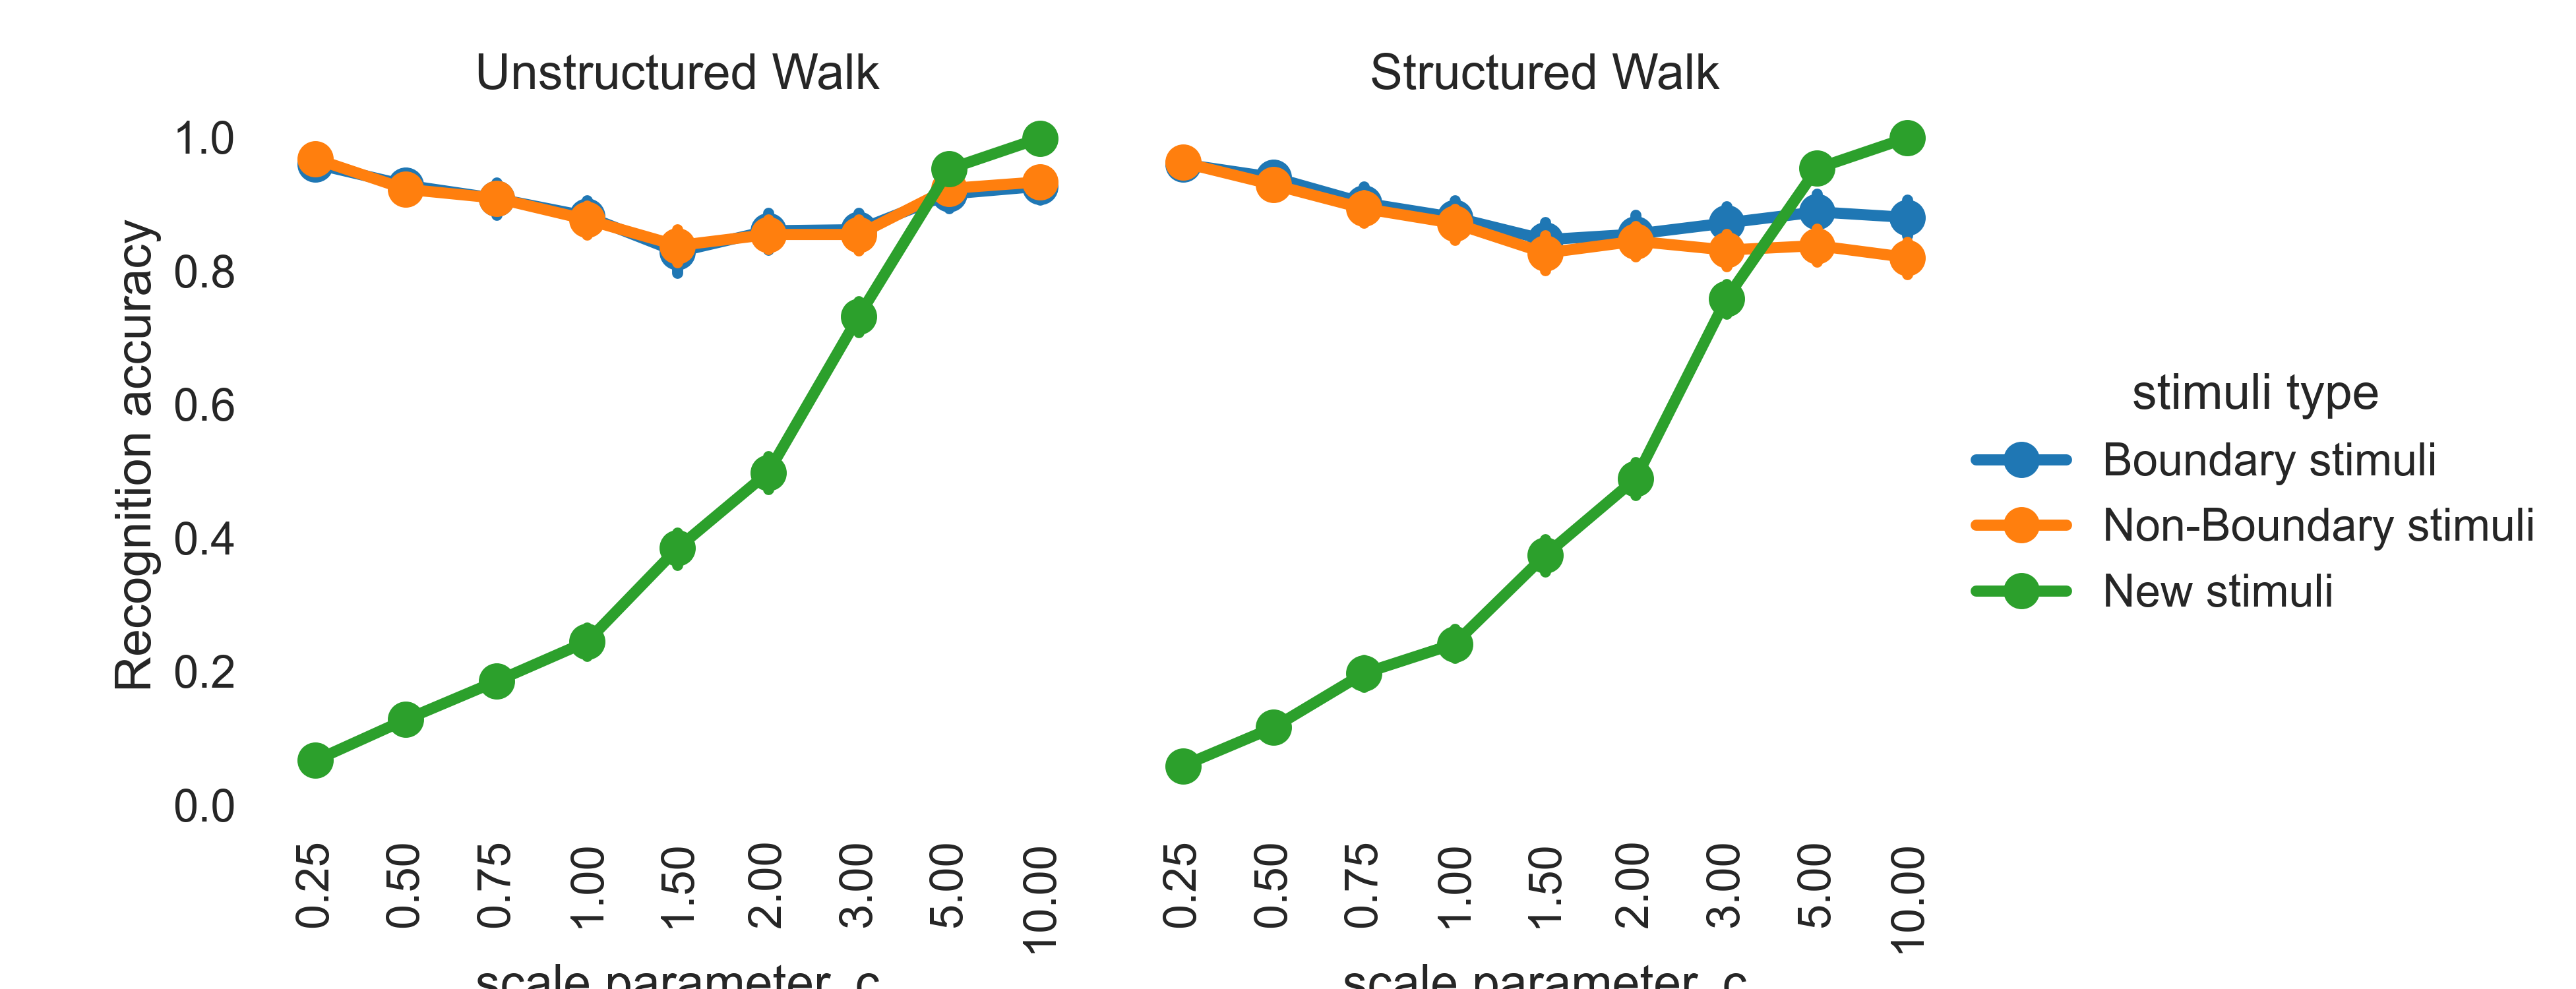
\includegraphics[width = \textwidth]{chapter_notebooks/chapter_3/figures/recog_memory_with_c.png}
    \caption{Simulated recognition memory test performances for walk lengths of 1 and walk lengths of 1000 on modular graph in Figure \ref{fig:modular_graph}. On average, recognition memory performance is expected to be better for boundary items than non-boundary items.}
    \label{fig:recog_memory_sims_with_c}
\end{figure}



\subsection{Methods}
\subsubsection*{Participants}
63 undergraduate students at the University of Massachusetts Amherst participated in this study. Participants were at least 18 years of age and were compensated via course credit. All procedures were approved by the University Institutional Review Board. \ac{Data from 6 participants who did not complete the study were discarded from further analyses. Participant sample size was not pre-determined via a statistical procedure but was a rough equivalent of previous studies \parencite{heusser2018perceptual}. All statistical inference in this article is done as probabilities of effects measured through posterior parameter estimates in Bayesian models.}

\subsubsection*{Stimuli}
\ac{Randomly polygon shapes were used as stimuli for this experiment. Each polygon consisted of 6 vertices. 2 vertices were randomly placed around the center of the screen with their X-Y coordinates drawn from univariate normal distributions with a standard deviation of 0.1 inches. Coordinates of the remaining four vertices were drawn from univariate uniform distributions between 0.1 and 0.3 inches. 300 polygons were generated and randomly chosen 60 (15 `old' and 45 `new') were used for each participant.}

\subsubsection*{Design and Procedures}
Participants were randomly assigned to either a structured exposure or an unstructured exposure group. The overall experimental procedures were the same across both groups. 

15 polygons were chosen randomly (from the set of 300) for each participant as `old' stimuli. At the beginning of the experiment, participants were asked to carefully study these polygons and to remember their orientation. During 750 exposure trials, separated into 3 blocks of 250, participants were presented these polygons one at a time and asked to judge whether the presented polygon was in its original orientation or rotated. \ac{Participants were provided feedback on their accuracy on each rotation judgment response and an on-screen score was maintained to motivate accurate responses.} Polygons were surrounded by a (purple, orange, or dark green) colored border to use for a source memory test.

Each polygon with its border was associated with a node in the modular graph in figure \ref{fig:exp2-design}. Order of polygons during exposure was determined by a participant's group. For 27 participants in the structured exposure group, the order of exposure was determined by a random walk through the modular graph (Figure \ref{fig:exp2-design}) \yk{where each subsequent node was determined based on a random choice of the connected node}. Exposure order for 30 participants in the unstructured group was determined by a random selection among the 15 items on each trial. 

\begin{figure}[ht]
    \centering
    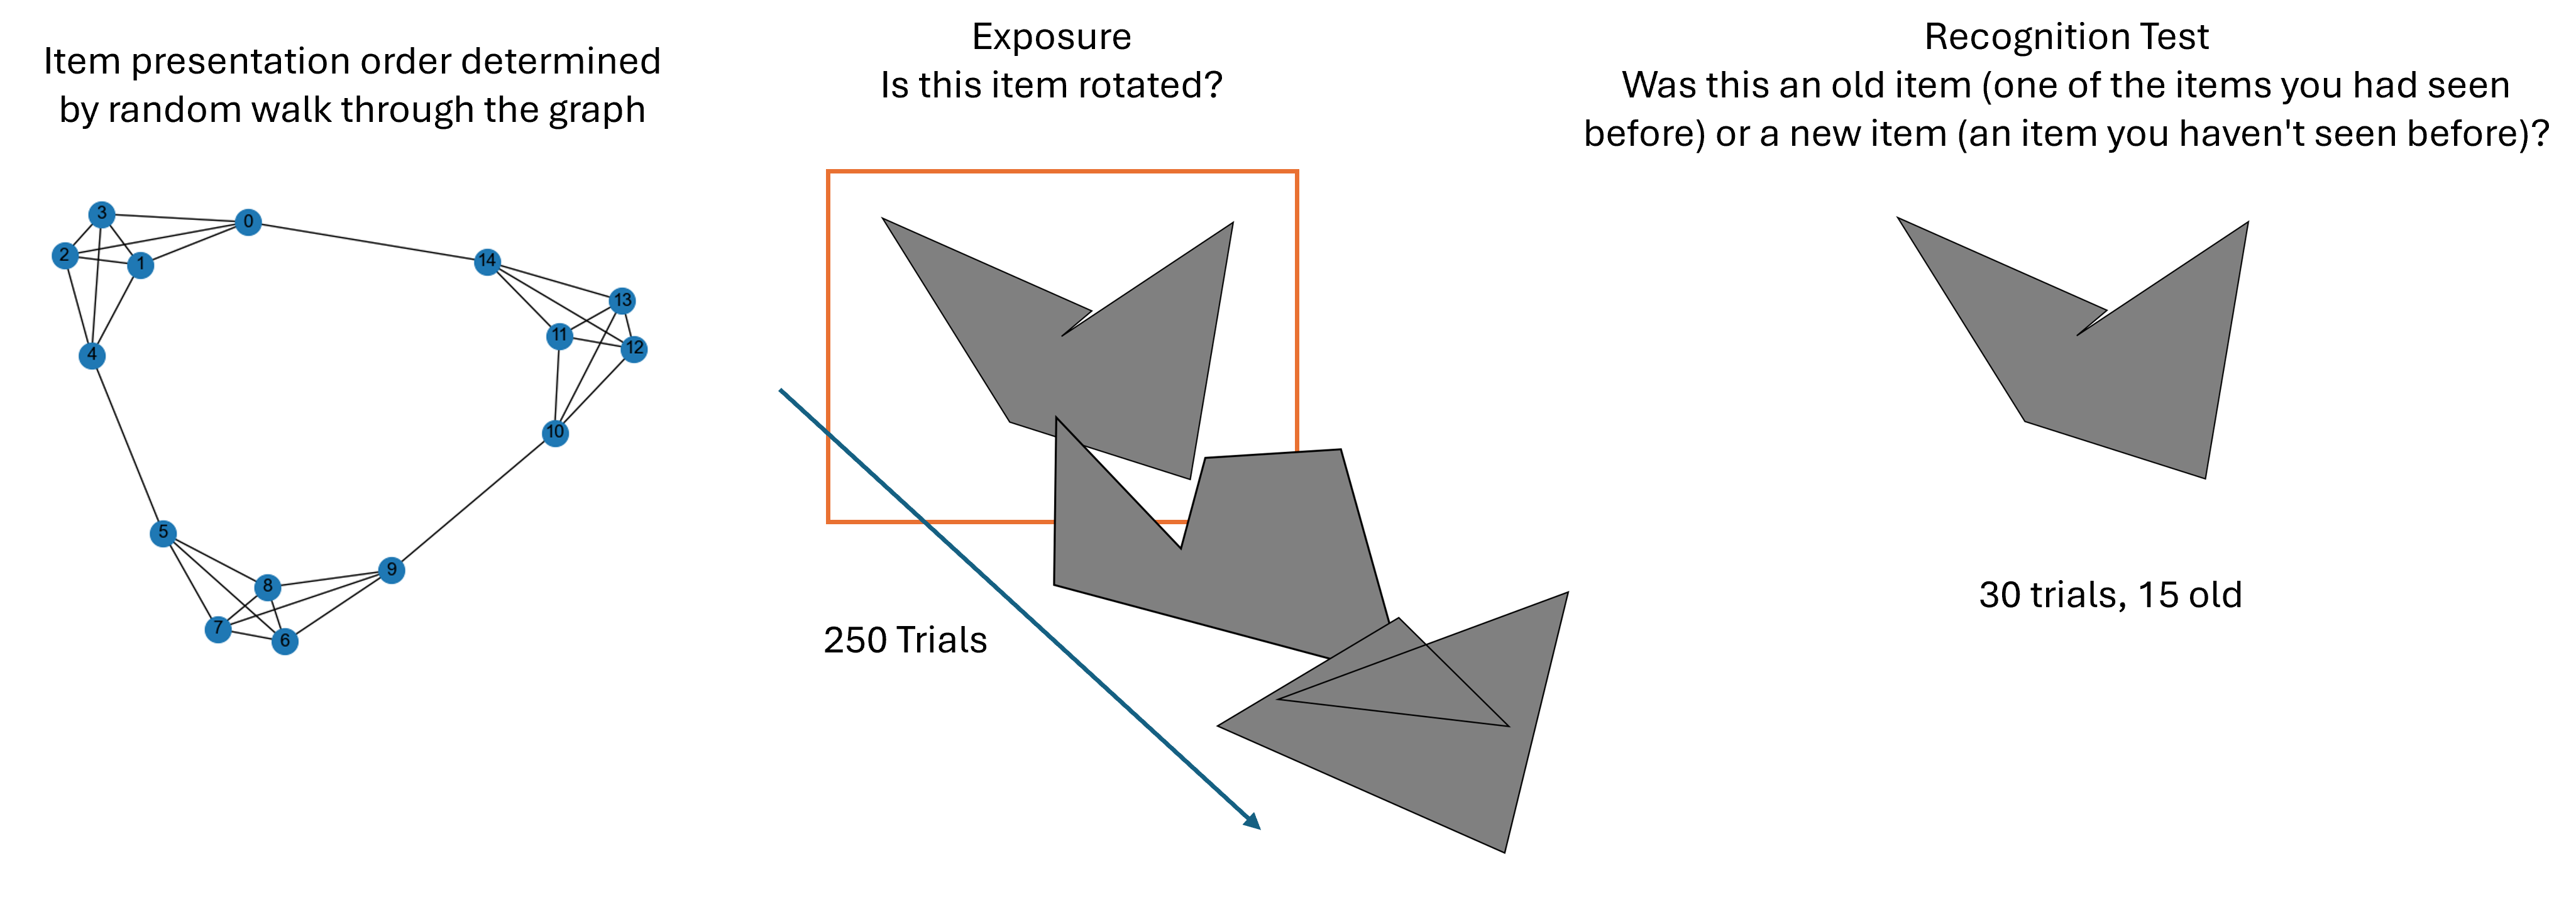
\includegraphics[width = \textwidth]{chapter_notebooks/chapter_3/figures/exp2_design.png}
    \caption{Design schematic for Experiment 2a. Three alternating blocks of exposure and recognition test were presented. A Stroop task was conducted prior to the final recognition test.}
    \label{fig:exp2-design}
\end{figure}

After each block of the exposure phase, participants went through a recognition memory test (Figure \ref{fig:exp2-design}). They were shown the 15 \yk{`old'} items from the exposure phase (in their original orientation) in addition to 15 new random polygon items (chosen from the set of 300) and were asked to determine whether each of these items was old or new. Order of presentation of old and new items was randomized during the recognition memory test. Of the three recognition tests, the final test was conducted after a short Stroop task to washout any effects of short term memory. 

After the final recognition memory test, participants went through a source memory test. Each of the 15 studied items were shown without the colored borders that surrounded them during exposure. Participants were asked to choose which of the three colored borders, provided as on-screen options, surrounded any particular item. This source memory task was added to provide an additional signal for memory in case of ceiling effects of recognition memory tasks. However, no analyses have been done on this source memory task. 


\subsection{Results}

As expected, accuracies for old stimuli increase with increased exposure (Figure \ref{fig:exp2-accuracies}, Table \ref{tab:acc-block-hdi} for a statistical test of \yk{increased accuracy and decreased response times over blocks}) whereas the response times decreased with more experience with the stimuli across blocks (Figure\ref{fig:exp2-rts}, Table \ref{tab:rt-block-hdi} for a statistical test). See Table \ref{tab:exp2-rt-accuracy-stats} provides the means and standard deviations for response times and accuracies \ac{during the exposure and recognition phases} across each block for all stimuli types for both conditions. \mh{Interestingly, overall accuracy of participants in the unstructured exposure condition is higher, than those in the structured exposure condition across all stimulus types. However, this effect apperas to be due to participant variability (See Table \ref{tab:acc-cond-hrl-hdi} for statistical results of a hierarchical model accounting for a varying effect of participants.)}. 

\begin{figure}
    \centering
    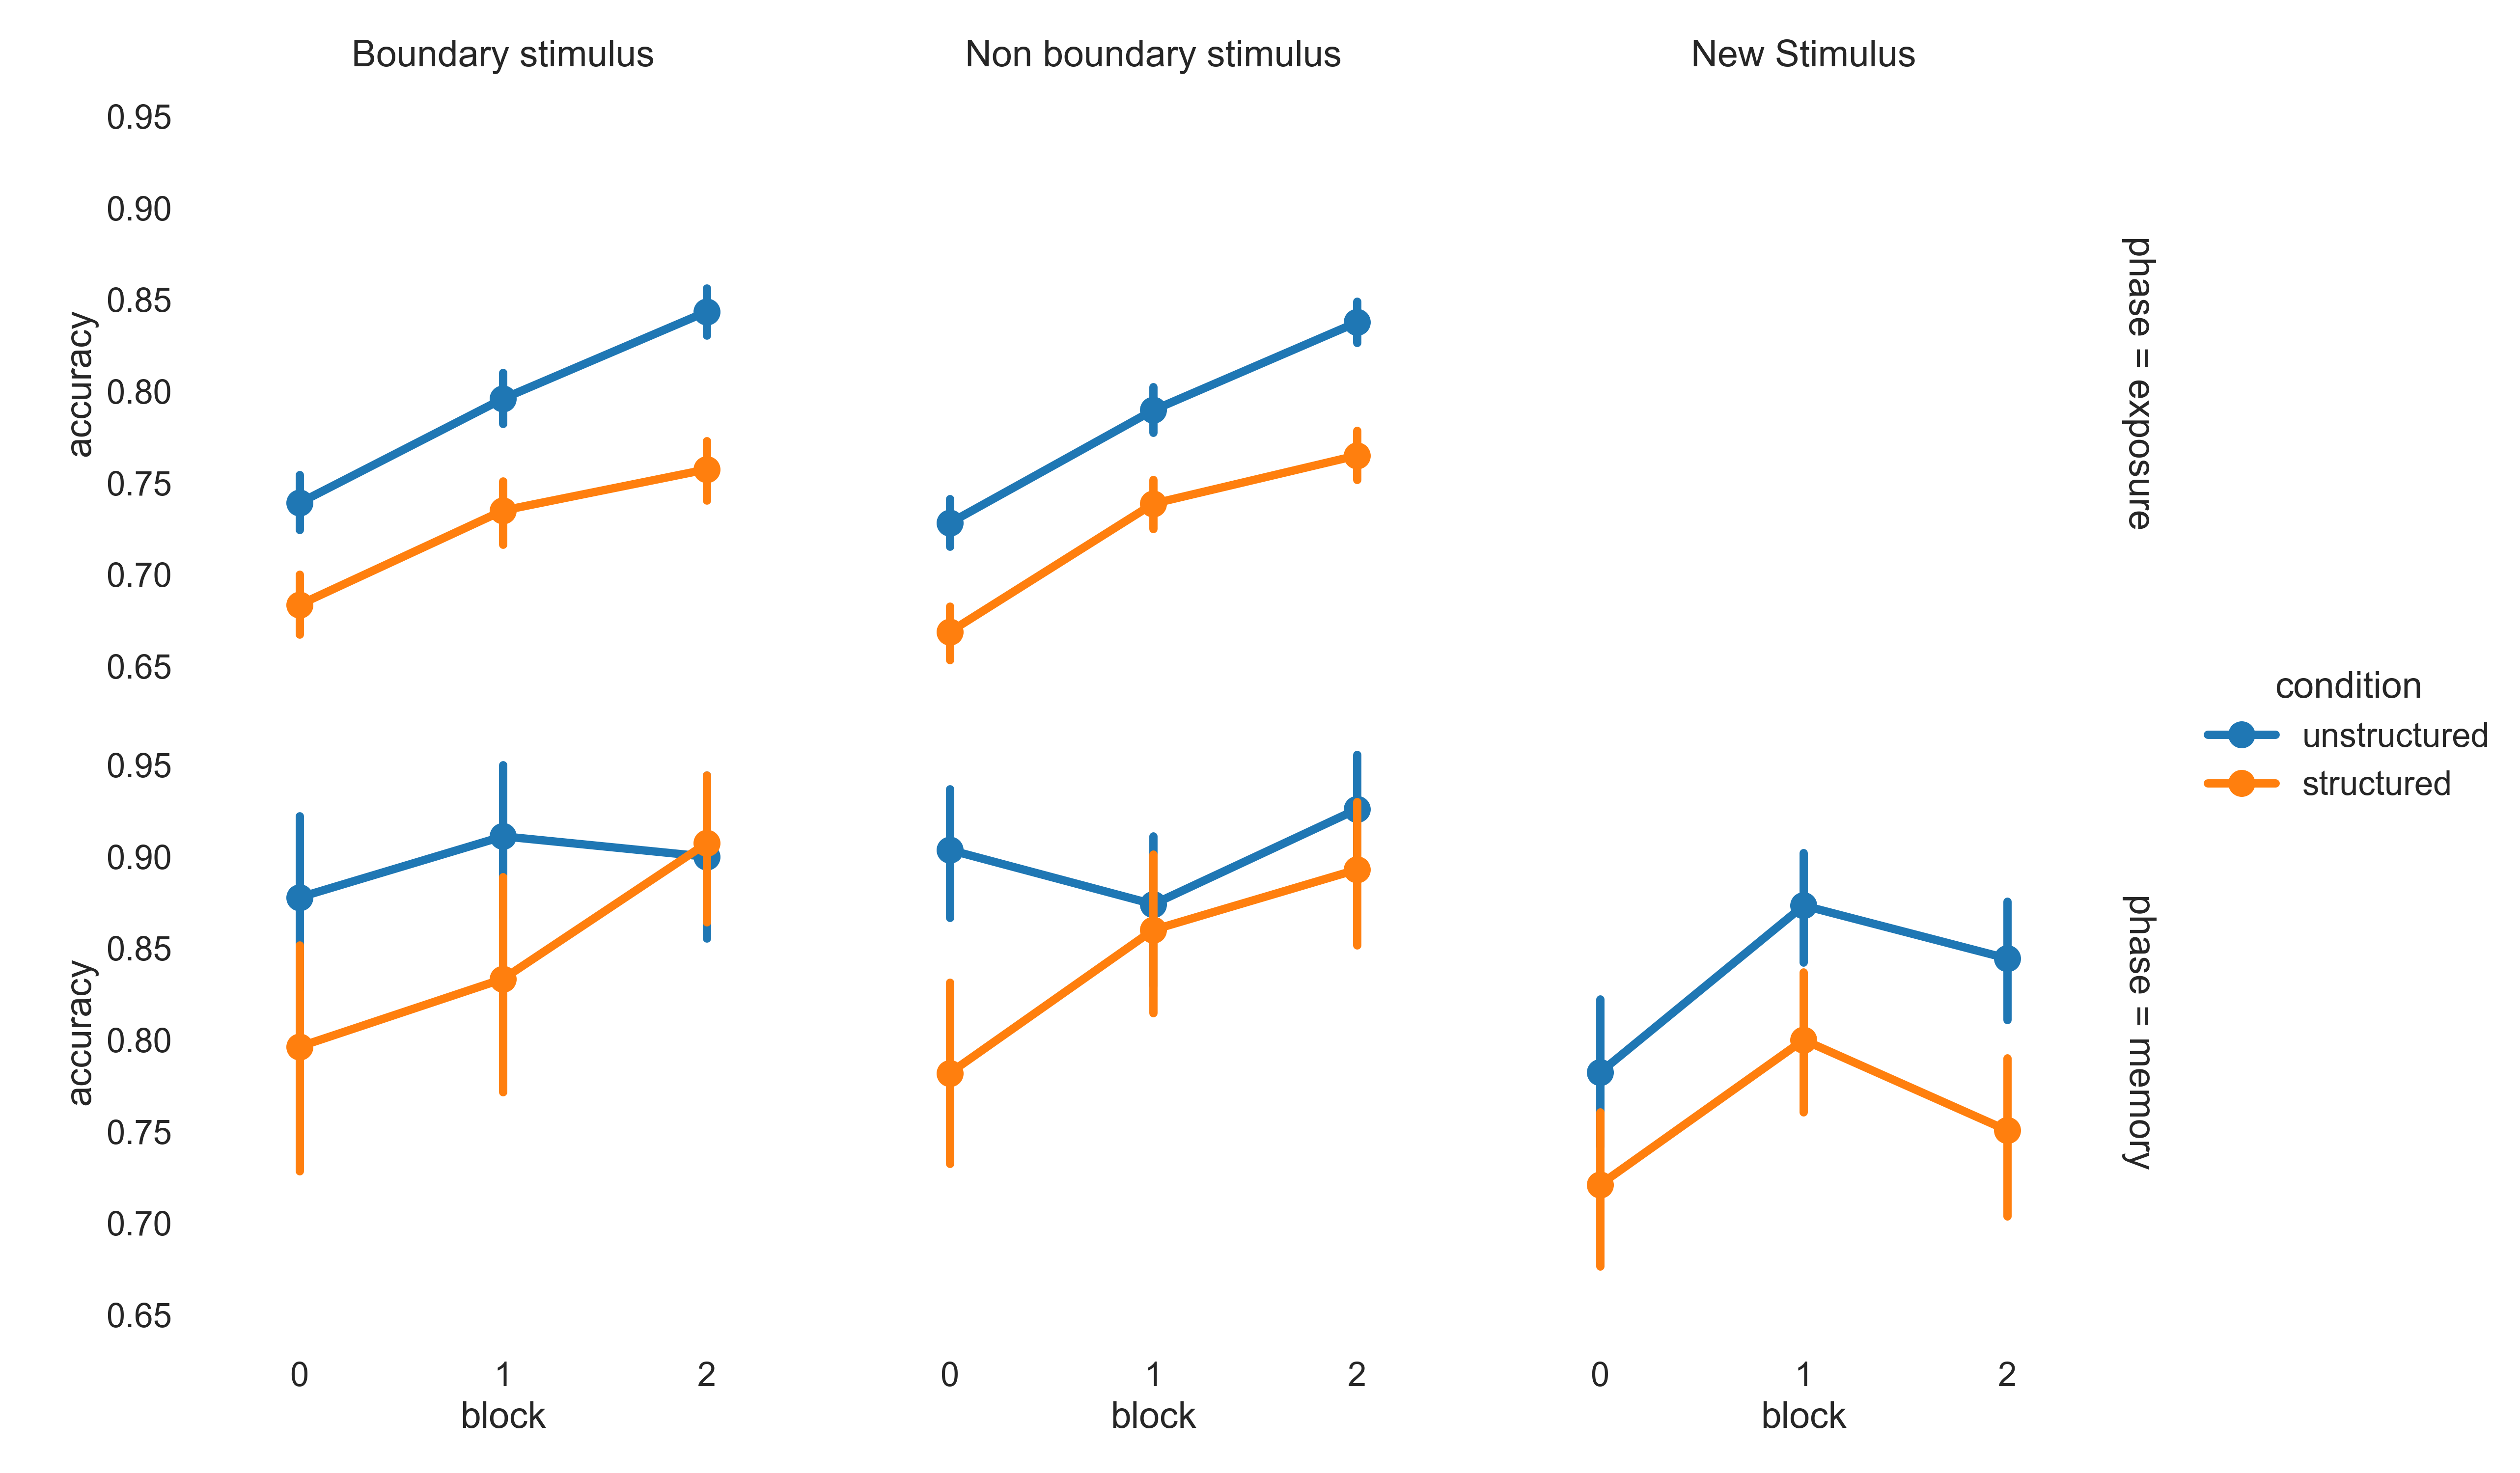
\includegraphics[width = \textwidth]{chapter_notebooks/chapter_3/figures/exposure_recog_accuracy_allphases.png}
    \caption{Mean accuracies for both participant groups (structured and unstructured) across blocks, for different stimulus types and phases of the experiment}
    \label{fig:exp2-accuracies}
\end{figure}


\begin{figure}
    \centering
    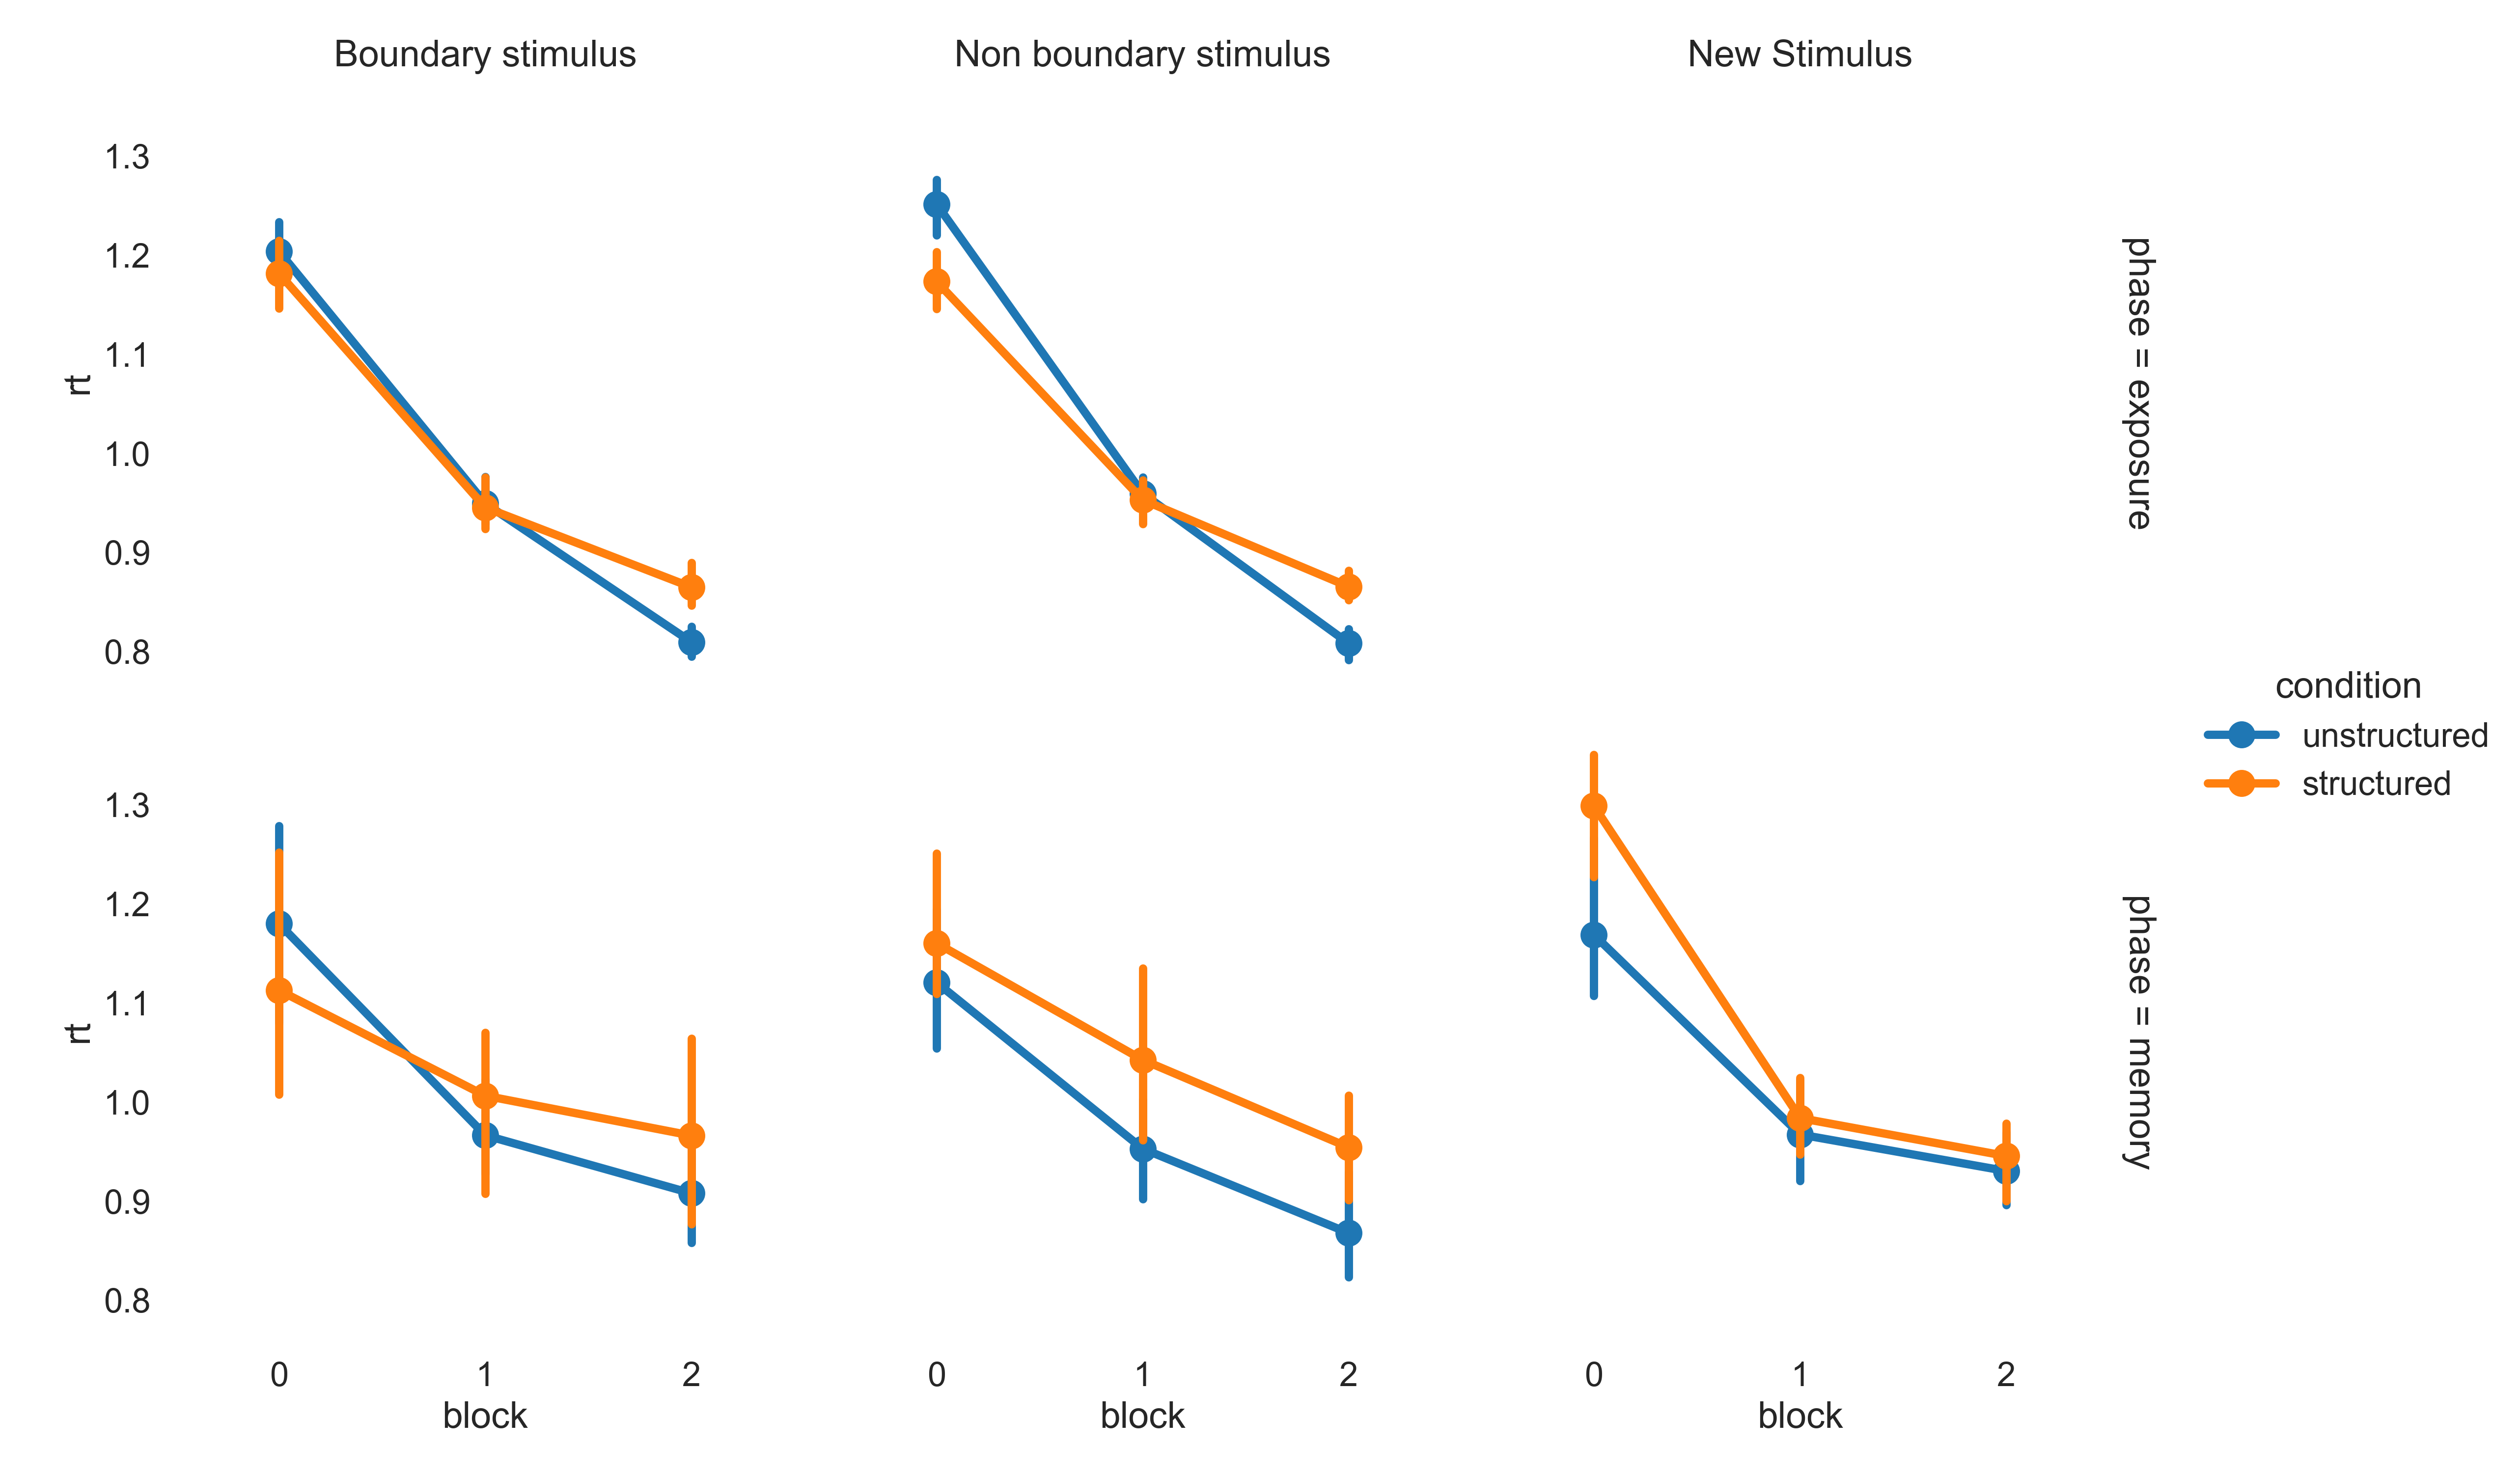
\includegraphics[width = \textwidth]{chapter_notebooks/chapter_3/figures/exposure_recog_rt_allphases.png}
    \caption{Median response times for both participant groups (structured and unstructured) across blocks, for different stimulus types and phases of the experiment}
    \label{fig:exp2-rts}
\end{figure}

To assess differences between stimulus types (boundary vs non-boundary) on recognition memory, a signal detection (SDT) model was first fit separately for items associated with boundary and non-boundary nodes. The model for boundary items describes the probability of responding `old' to old boundary stimuli relative to new stimuli. Similarly, the model for non-boundary items describes the probability of responding `old' to old non-boundary items relative to new stimuli. A participant intercept term allows for each participant to have their own decision criterion. \mh{Finally, accuracy at exposure was included as a factor in the SDT model to account for differences in encoding accuracy. Exposure accuracy factor for old items was computed by averaging the rotation judgment accuracy for each of the old items in the block immediately before the recognition memory block. For new items, this factor was computed by averaging the rotation judgment accuracy for all exposure items in the exposure block before that recognition phase.} The SDT model can be described as: 

\begin{equation}
    \begin{aligned}
        accuracy\ exposure \sim \mathcal{N}(0, 13.87) \\
        true\ old | condition \sim Normal(mu: 0.0, Half\mathcal{N}(sigma: 5.5)) \\ 
        participant\ criterion \sim \mathcal{N}(0, Half\mathcal{N}(sigma: 11.5)) \\
        \mu = (true\ old | condition) + accuracy\ exposure + participant\ criterion \\ 
        p(resp\ old) \sim Bernoulli(\mu)        
    \end{aligned}
\end{equation}


% The model fits relatively well as shown in figure \ref{fig:exp2-sdt-fits}.

% \begin{figure}
%     \centering
%     \label{fig:exp2-sdt-fits}
%     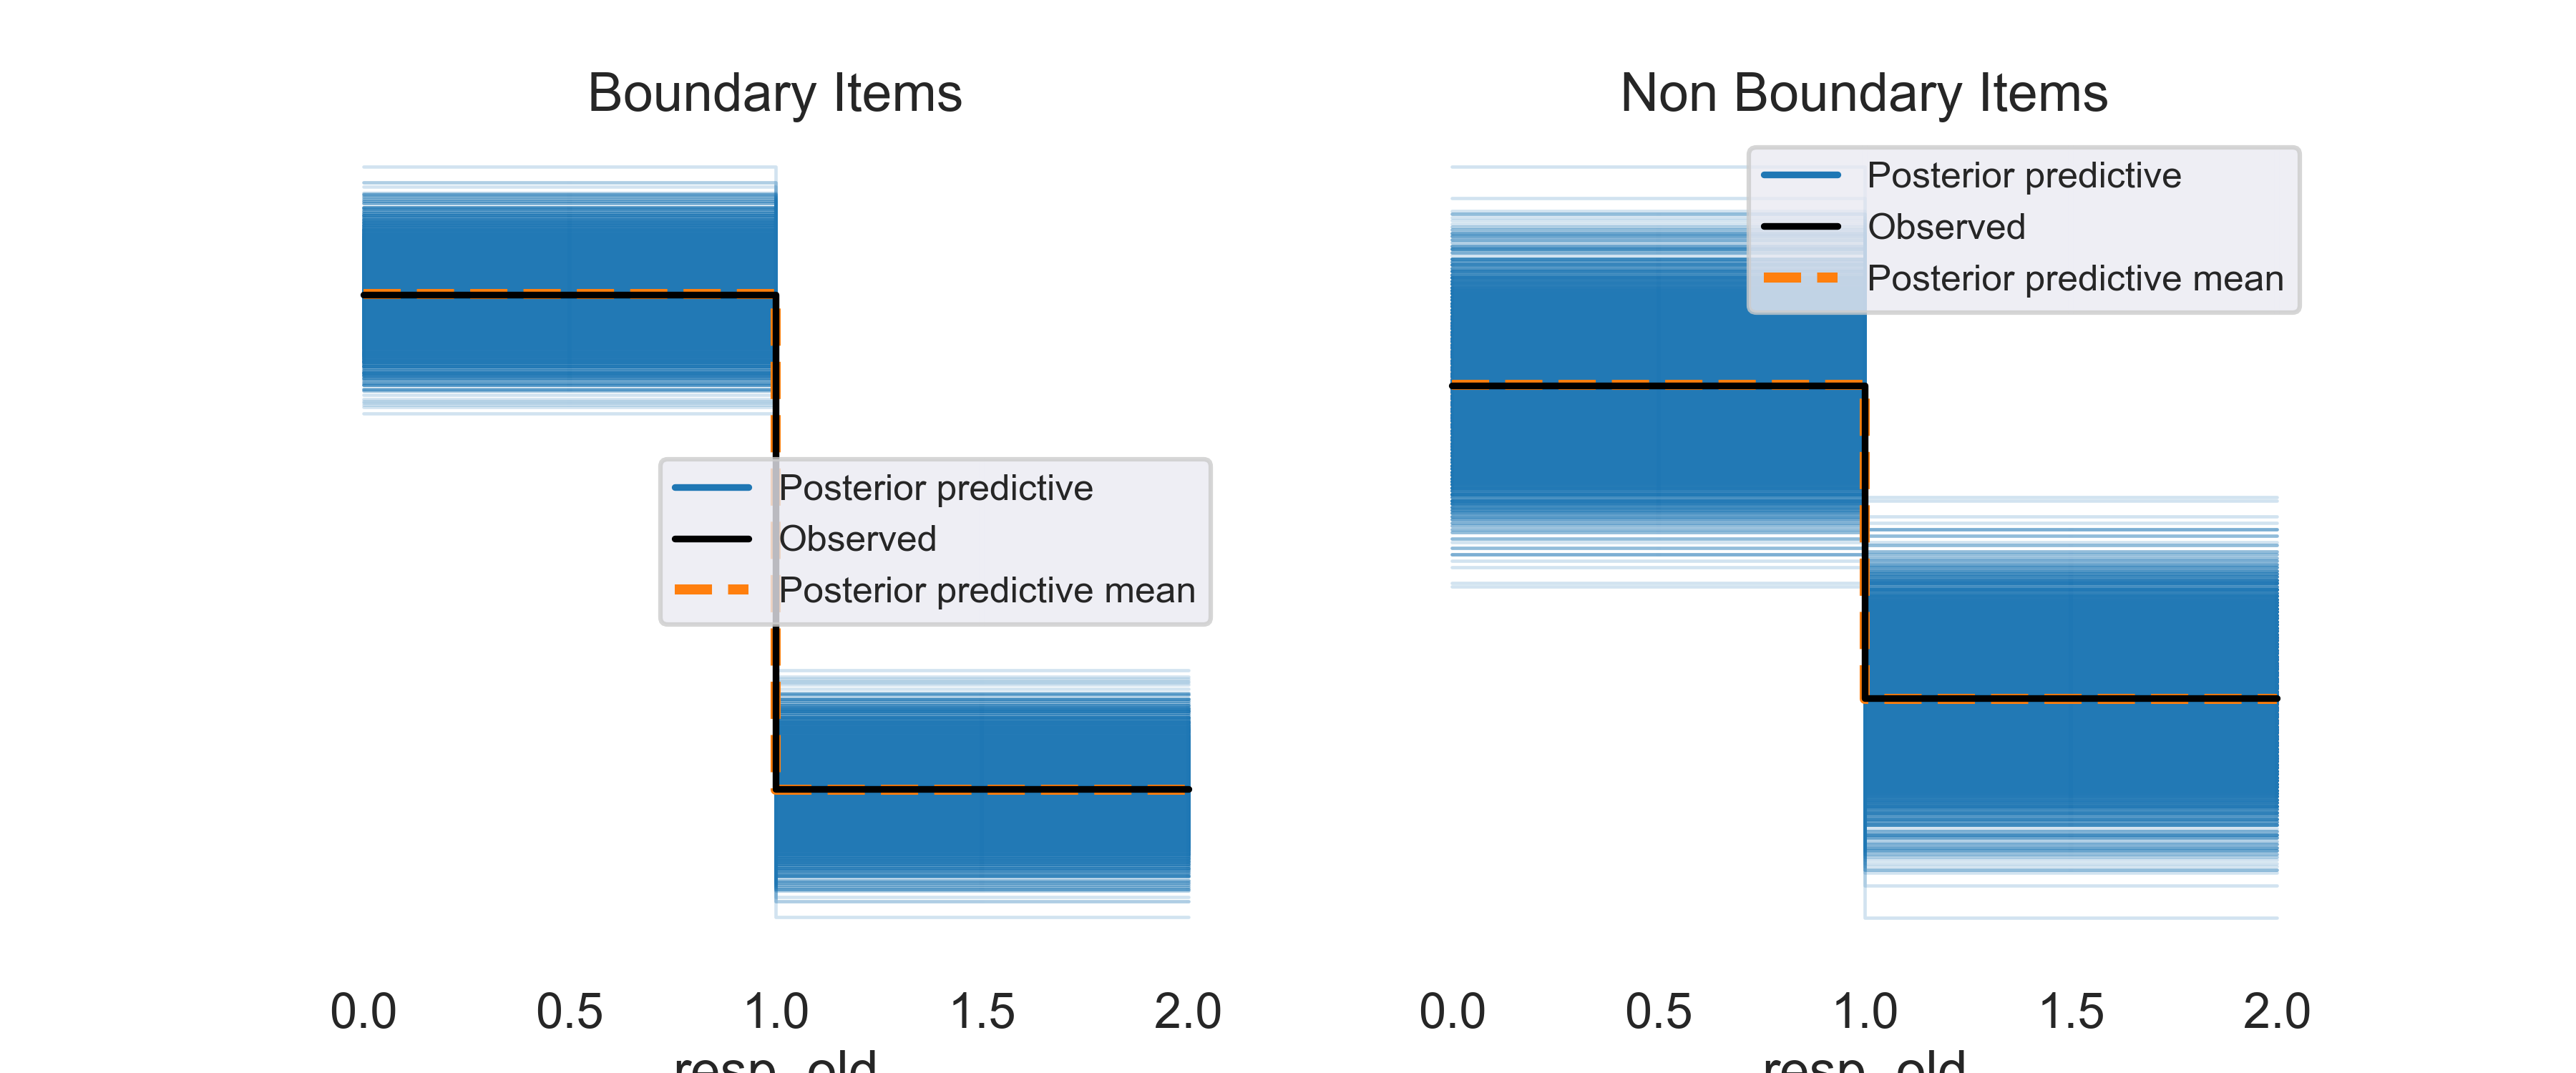
\includegraphics[width = \textwidth]{chapter_notebooks/chapter_3/figures/ppc_sdt_model.png}
%     \caption{SDT Model Posterior Predictive Distributions for boundary and non boundary items}
% \end{figure}

$d'$, the coefficient for $true\ old | condition$ in the linear model above, measures the distance between distributions of old and new items. Parameter estimates of $d'$ for structured relative to unstructured for boundary and non-boundary nodes for the final recognition block are shown in figure \ref{fig:sdt-params}. Parameter statistics are reported in appendix tables \ref{tab:exp3-bayesmodel-boundary-sdt} and \ref{tab:exp3-bayesmodel-nonboundary-sdt}

\begin{figure}
    \centering
    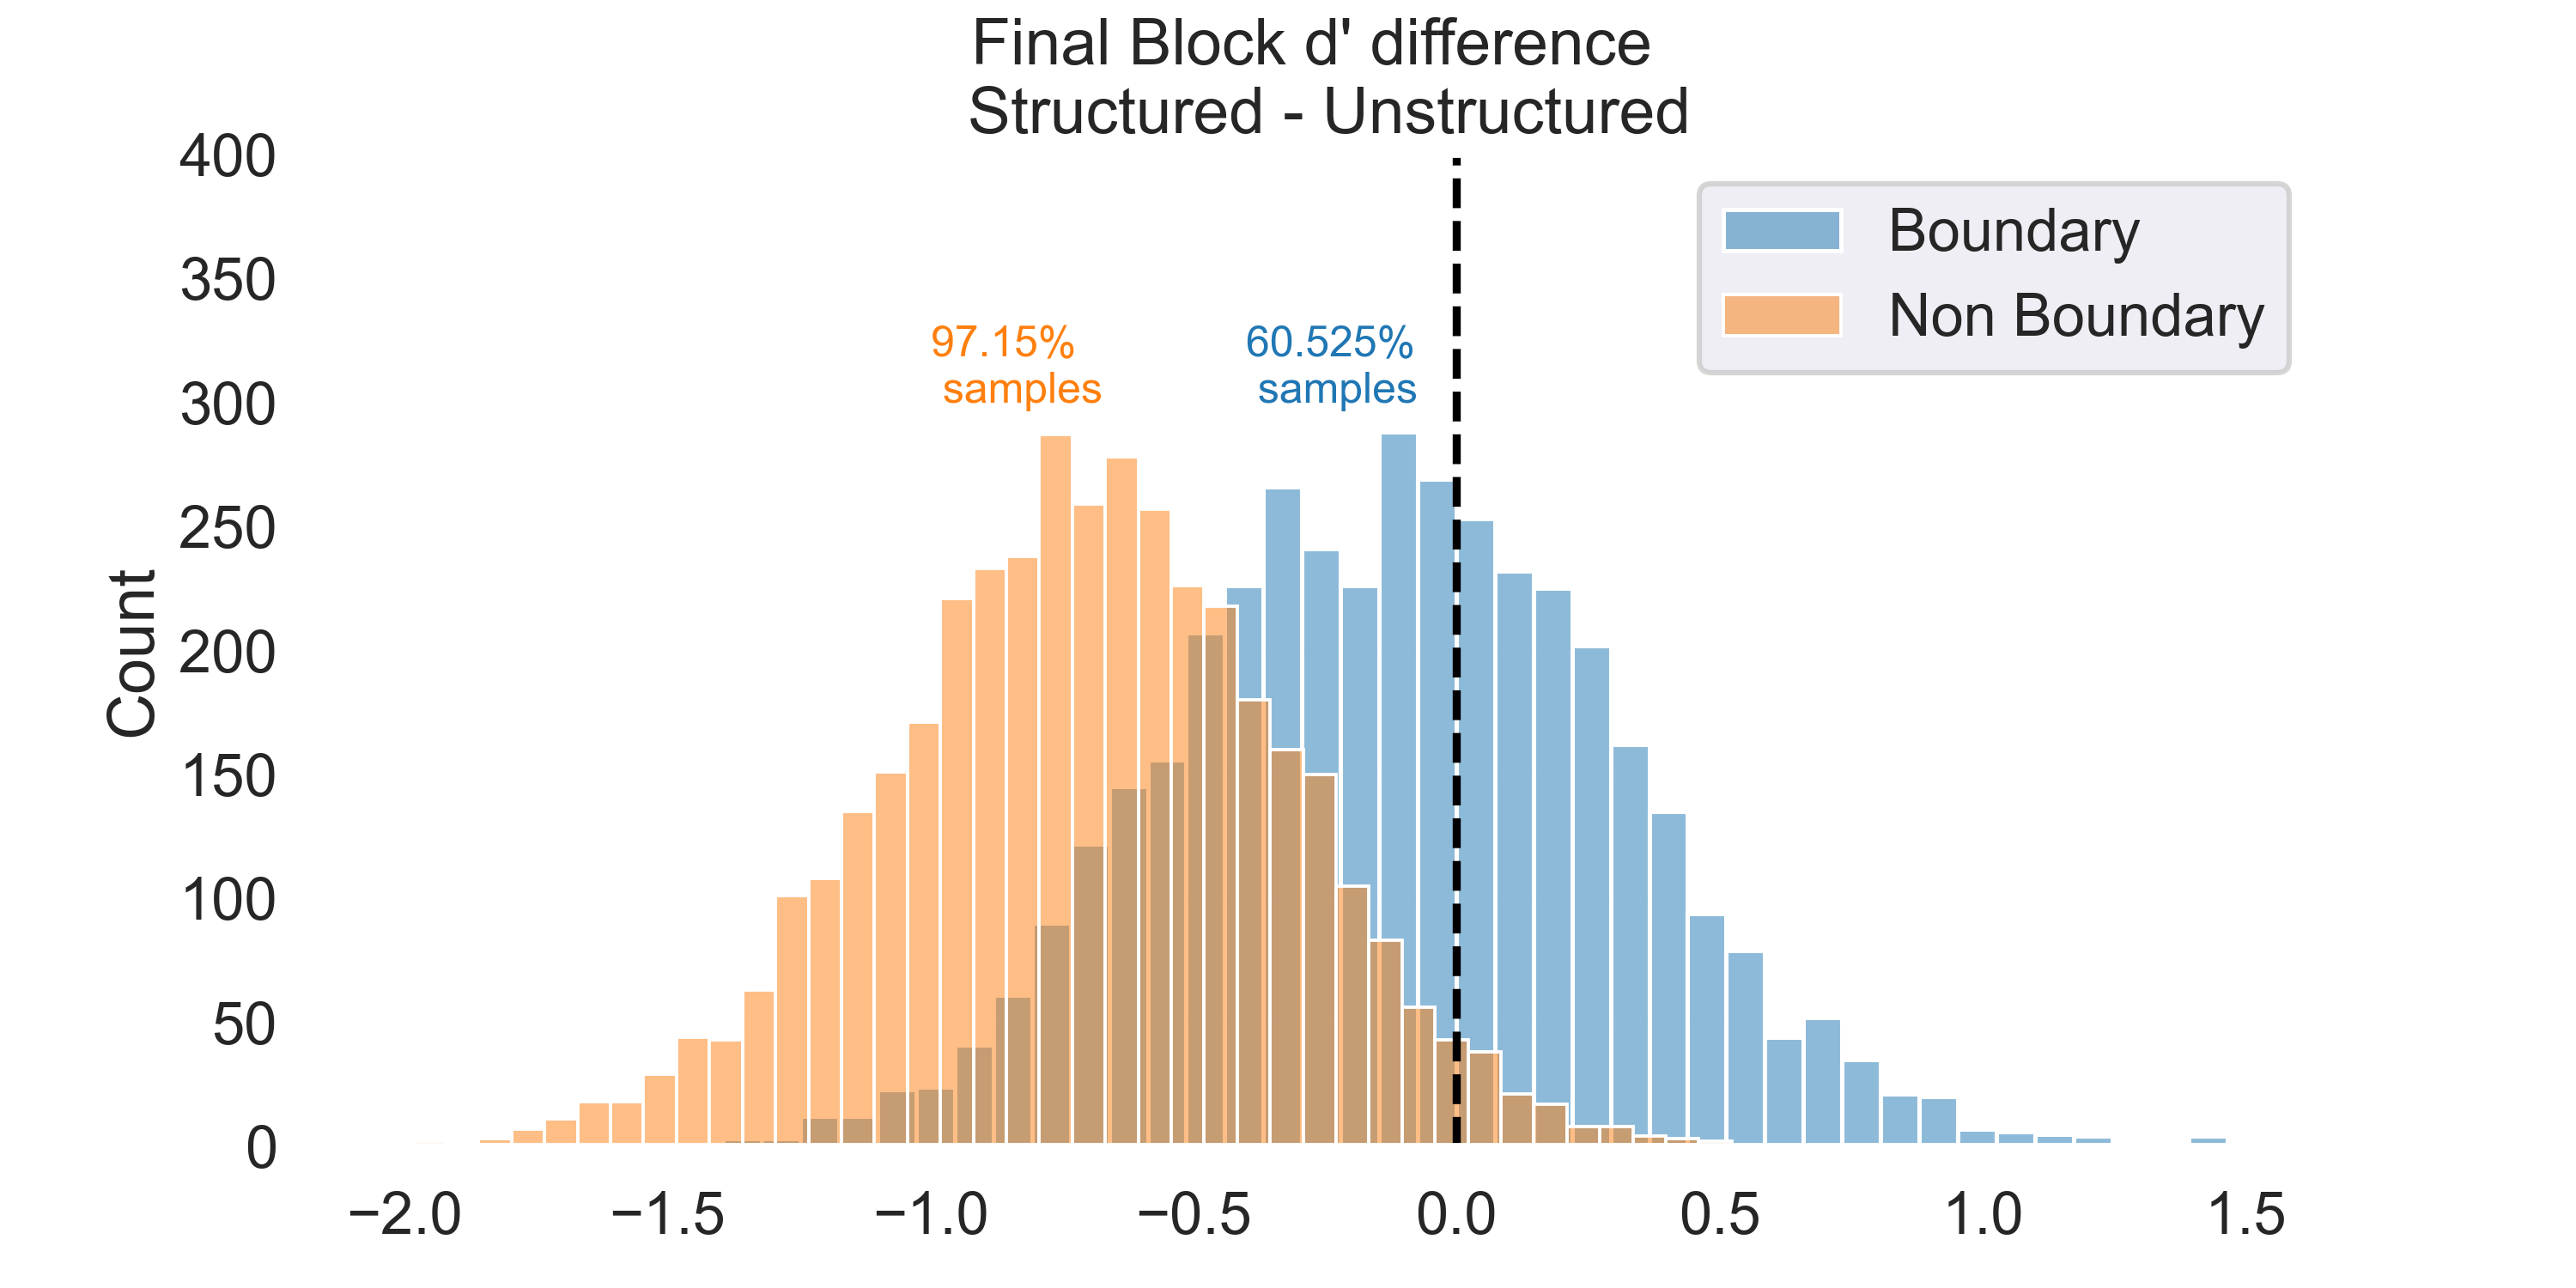
\includegraphics[width = \textwidth]{chapter_notebooks/chapter_3/figures/sdt_d_results.png}
    \caption{Differences in $d'$ for models fit to separately boundary and non-boundary nodes for both structured and unstructured exposure conditions}
    \label{fig:sdt-params}
\end{figure}

The SDT modeling implies that while there are no differences in recognition memory for boundary nodes based on exposure (60\% of posterior samples of the difference between structured an unstructured conditions below 0), non-boundary nodes seem to become less recognizable under structured exposure condition (97\% of the posterior samples of the difference between structured and unstructured conditions are below 0). 

\subsubsection*{Diffusion Modeling}
The SDT model used above fails to account for ceiling effects -- accuracy for old items is near perfect or could have reached an asymptote. The SDT model was also fit separately to derive $d'$ for boundary and non-boundary items, thus losing shared variability within participants.

To be able to account for ceiling effects in recognition accuracy, we can use additional information available in the form of response times during the recognition memory task. For example, for participants equally accurate in recognizing boundary and non-boundary participants, being able to recognize boundary items faster may provide additional evidence for better memorability of these items relative to slower recognized non-boundary items. Figure \ref{fig:exp2-rts} shows median response times across three blocks of recognition test. 

To understand recognition memory differences between the boundary and non-boundary items in context of response accuracy and response time distributions, we use the Drift Diffusion Model (DDM, Figure \ref{fig:ddm-model}). The DDM, which falls under a class of sequential sampling models, has been a widely successful model in modeling two-choice tasks in recognition memory \parencite{ratcliff2004diffusion, ratcliff2022discriminating, starns2014using, starns2014validating, ratcliff2009modeling}. 

\begin{figure}[ht]
    \centering
    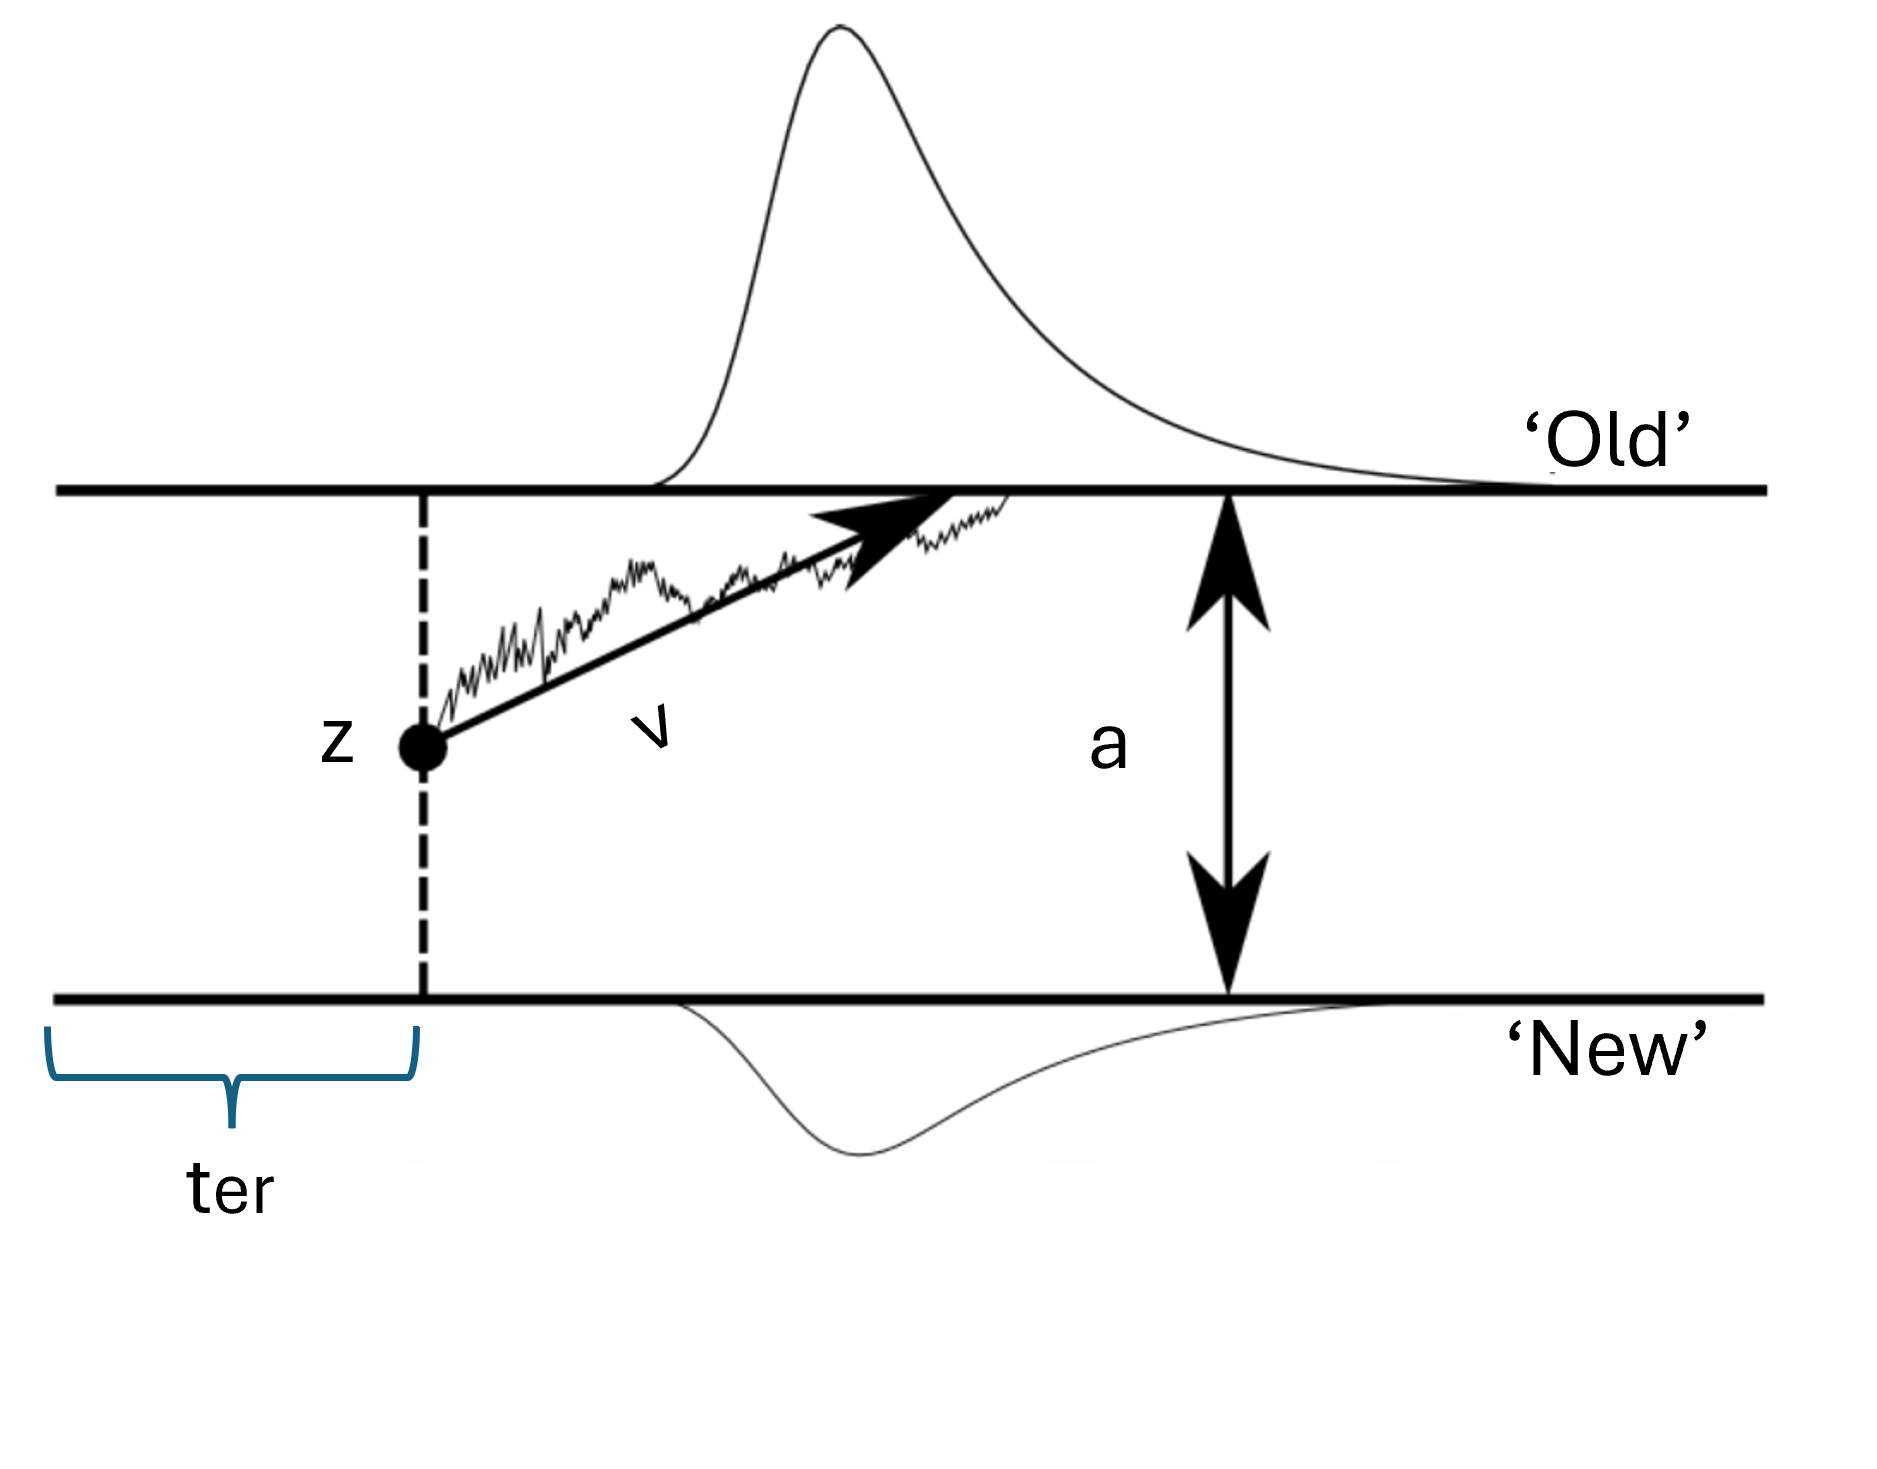
\includegraphics[width = 0.75\textwidth]{chapter_notebooks/chapter_3/figures/ddm.png}
    \caption{The Drift Diffusion Model of Choice Response Times for Old/New recognition memory tasks.}
    \label{fig:ddm-model}
\end{figure}

Briefly, the DDM assumes that at choice time, evidence from two presented options accumulates sequentially over time towards one of the two boundaries. For a previously studied item presented at test, the evidence from the item accumulates slowly towards the `old' boundary whereas for a non-studied item, the evidence accumulates towards the `new' boundary. The rate of evidence accumulation is controlled by the drift rate parameter, $v$. Participants may be biased towards making an old or a new response at test; this bias is measured by the starting point parameter, $z$. The boundary separation between the two responses is modeled by a parameter $a$. Finally, the observed response consists of cognitive processes not affiliated with decision making (such as time it takes to visually process the test item, time for the motor systems to click the relevant key) which are modeled by a non-decision time parameter $t_{er}$. \footnote{Note that this version of the DDM is a simplified model. More complex DDMs account for trial-to-trial variability in each parameters as well.} 

Prior work has shown that memory strength of previously studied items impacts the drift rate towards old/new responses \parencite{ratcliff2004diffusion,ratcliff2022discriminating}. A higher drift rate parameter implies a stronger match to memory which leads to a quicker accumulation of evidence towards the `old' response boundary. Similarly, a stronger mis-match to memory (as measured by the higher drift rate parameter) allows for a quicker accumulation of evidence towards the `new' response boundary \parencite{ratcliff2004diffusion,ratcliff2022discriminating}. 

The DDM thus allows us to circumvent ceiling effects by modeling response time distributions (\yk{as faster accurate trials may reflect better memory than slower accurate trials}) and estimate whether boundary items are indeed remembered better than non-boundary items in the structured exposure or whether the effect is driven by worse-remembered non-boundary items (\yk{as faster accurate non-boundary stimuli recall may reflect better memory than slower accurate non-boundary stimuli}). 

For the recognition task in the current study, the DDM was parameterized as follows: 
\begin{equation}
    \begin{aligned}
        v \sim 0 + node type:condition:block + accuracy\ exposure \\
        z \sim 0 + block \\
        a \sim 0 + condition:block \\
        t_{er} = 0.25
    \end{aligned}
\end{equation}

The fixed value of the non decision time parameter $t$ was derived by first fitting the DDM over a range of possible $t$ values (i.e. a grid search) and picking value with the best fitting model in that range. DDM models were fit using the HSSM package \parencite{fengler2022beyond}. \footnote{Unfortunately the non decision time parameter is too difficult to fit -- this is a known problem with the HSSM package} 

\paragraph*{DDM Results}
The modeling framework above allows incorporating response times during recognition memory tasks. In particular, if an item is quickly and accurately recognized as old or new, in addition to good accuracy, such recognition would result into faster reaction times. This effect is captured by the drift rate parameter of the DDM. 

\begin{figure}
    \centering
    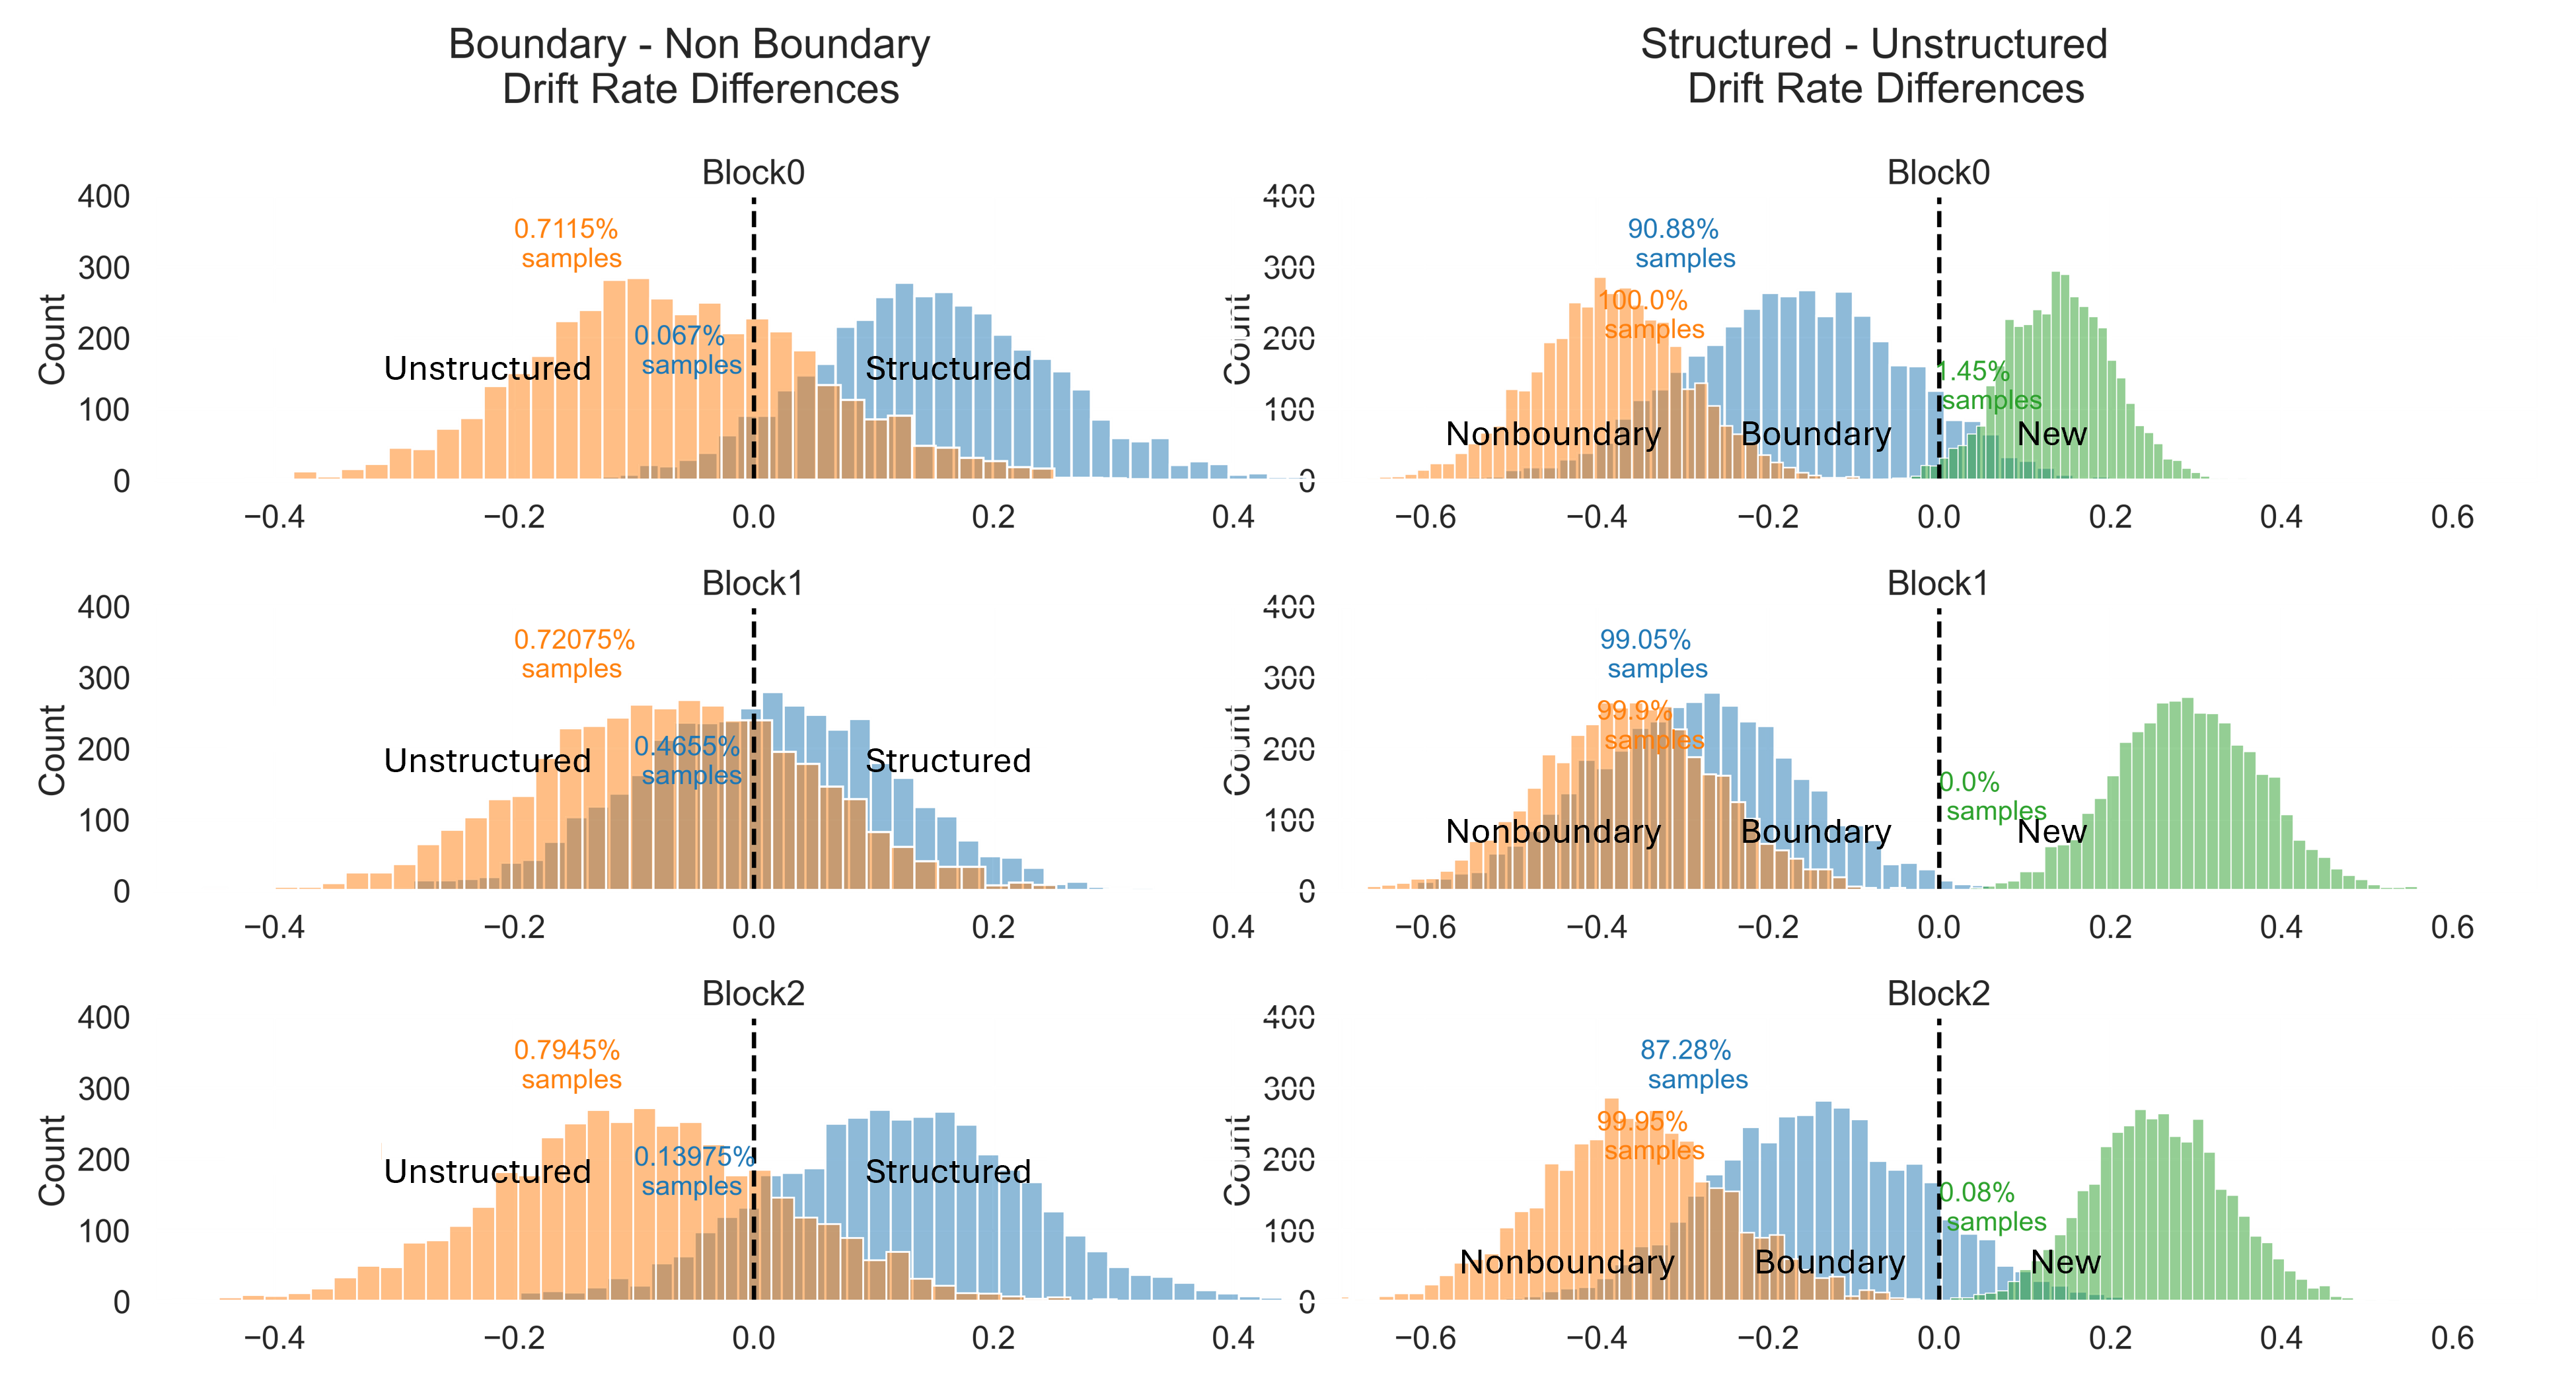
\includegraphics[width = \textwidth]{chapter_notebooks/chapter_3/figures/ddm_vdiff_comb.png}
    \caption{Drift rate differences. \textit{Left Panel.} Differences between boundary and non-boundary nodes for structured and unstructured exposure conditions. \textit{Right Panel} Differences between drift rates between structured and unstructured conditions for each type of recognition memory stimulus. Figure text over each difference distribution depicts the proportion of posterior samples above 0.}
    \label{fig:ddm-drift-rates}
\end{figure}

Figure \ref{fig:ddm-drift-rates} shows the differences between drift rate parameters. \mh{The modeling framework introduced earlier used SR to derive an estimate of entropy for each stimulus depending on its boundary or non-boundary role in the modular graph of Figure \ref{fig:exp2-design}. Node entropy further was assumed to enhance memory strength of the stimulus associated with that node such that, on average, stimuli that are associated with boundary nodes are expected to be remembered better than those associated with non-boundary nodes for participants who are exposed to a structured random walk. No such difference is expected for participants exposed to an unstructured walk. We thus expect that the drift rate, as proxy for memory strength, would be higher for boundary nodes for structured random walk participants than for non-boundary nodes. This difference in boundary vs non-boundary item drift rates should be relatively higher for participants exposed to the structured condition than for the participants in our control condition; those exposed to the unstructured walk.} 

The left panel in Figure \ref{fig:ddm-drift-rates} shows that, as expected, boundary nodes have a higher drift rate than non-boundary nodes in the structured conditions relative to the unstructured conditions. \mh{This difference is more apparent in the first and the final block with 93.3\% and 86.02\% of posterior samples of the differences in drift rate being above 0 for structured condition whereas 28.85\% and 20.55\% of samples above 0 for unstructured condition. This difference disappears for the middle block (53.45\% samples for the structured condition and 27.92\% for unstructured) likely due to recognition test presented immediately after exposure and at this point participants have been exposed to the old stimuli for 500 trials. The difference likely reappears in the final block due to the Stroop distractor task administered before recognition test.}

\mh{The right panel shows the same effect within conditions. New items appear to have better drift rates than old items in the structured condition than the unstructured conditions across all blocks. While drift rates for `old' items were generally lower for the structured condition (relative to the unstructured condition), they were higher for the boundary nodes than non-boundary nodes indicating that even when stimuli at boundary nodes are remembered worse in structured condition than those at boundary nodes in the unstructured condition, they are still remembered better than the stimuli at non-boundary nodes in the structured condition. See Table \ref{tab:exp3-ddm-params} for full parameter statistics of the DDM.}

\subsection*{Interim Conclusion}
\ac{Findings in the first experiment in the current work show that similar to explicitly operationalized boundaries, implicitly operationalized boundaries are remembered better than non-boundaries. Furthermore, these improved boundary memory effects can be supported by an SR-derived entropy formulation. Stimuli associated with boundary nodes carry more information about the graph structure than those at non-boundary nodes. This additional information leads to slower reaction times (Chapter \ref{chapter-2-walk-lengths-modulate-statistical-learning}) and improved memory for those stimuli.}


\section{Experiment 2b: Boundary Distance Effects}
\subsection*{Modeling Boundary distance effects}
Another replicated finding in explicitly operationalized event boundary literature is an apparent increased separation of events across boundaries \parencite{horner2016role,brunec2018boundaries,dubrow2013influence, ezzyat2011constitutes, heusser2018perceptual}. This separation of events across boundaries helps shape narratives in long term memory \parencite{clewett2019transcending}.

It is unknown, however, whether the increased temporal separation across event boundaries generalizes to boundaries operationalized implicitly as well. Context models such as SR provide a mechanism to directly estimate perceived distance between events. Specifically, each cell in the SR matrix $M(s, s')$ indicates the future expected visit probabilities from state $s$ to state $s'$. Under the assumption that states closer to the current state are visited more often in a random walk than state farther, the probability $M(s, s')$ provides a direct estimate \ac{of probability of seeing node $s$ from node $s'$ and an hence an indirect estimate of the perceived distance} from node $s$ to $s'$. 

\begin{figure}[ht]
    \centering
    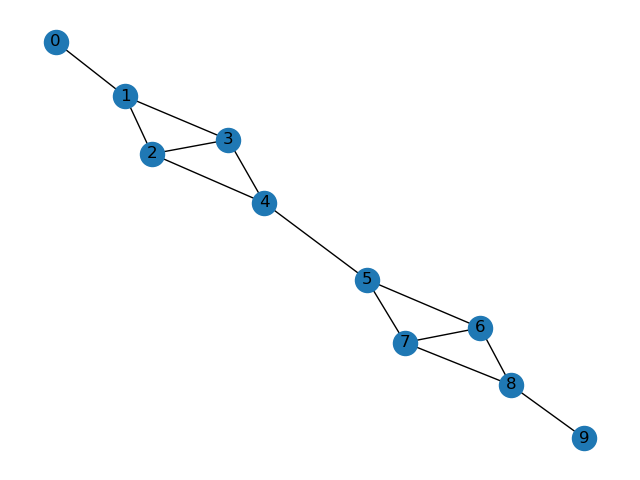
\includegraphics[width = \textwidth]{chapter_notebooks/chapter_3/figures/two_module_graph.png}
    \caption{Two module graph used for distance judgments.}
    \label{fig:two_module_graph}
\end{figure}

To test whether cross boundary events are perceived to be farther from each other relative to within-boundary events graph in Figure \ref{fig:two_module_graph} is used. \ac{This modular graph provides some desirable properties for a distance judgment task such as fewer stimuli to remember, and remote nodes along with non-remote, non-boundary nodes with same number of connections}. The key transitions of interest that are compared in this graph are transitions at equal distances (\ac{distance defined by the number of connections needed to be traversed to reach a node from another node}). Below I specify example transitions at 3 different distances however, for simulations and the experiment, all symmetrical transitions at those distances were tested. 
\begin{itemize}
    \item $0 \leftrightarrow 4$ vs $1 \leftrightarrow 5$ at distance 3. 
    \item $1 \leftrightarrow 4$ vs $2 \leftrightarrow 5$ at distance 2. 
    \item $2 \leftrightarrow 4$ vs $5 \leftrightarrow 4$ at distance 1. 
\end{itemize}

\begin{figure}
    \centering
    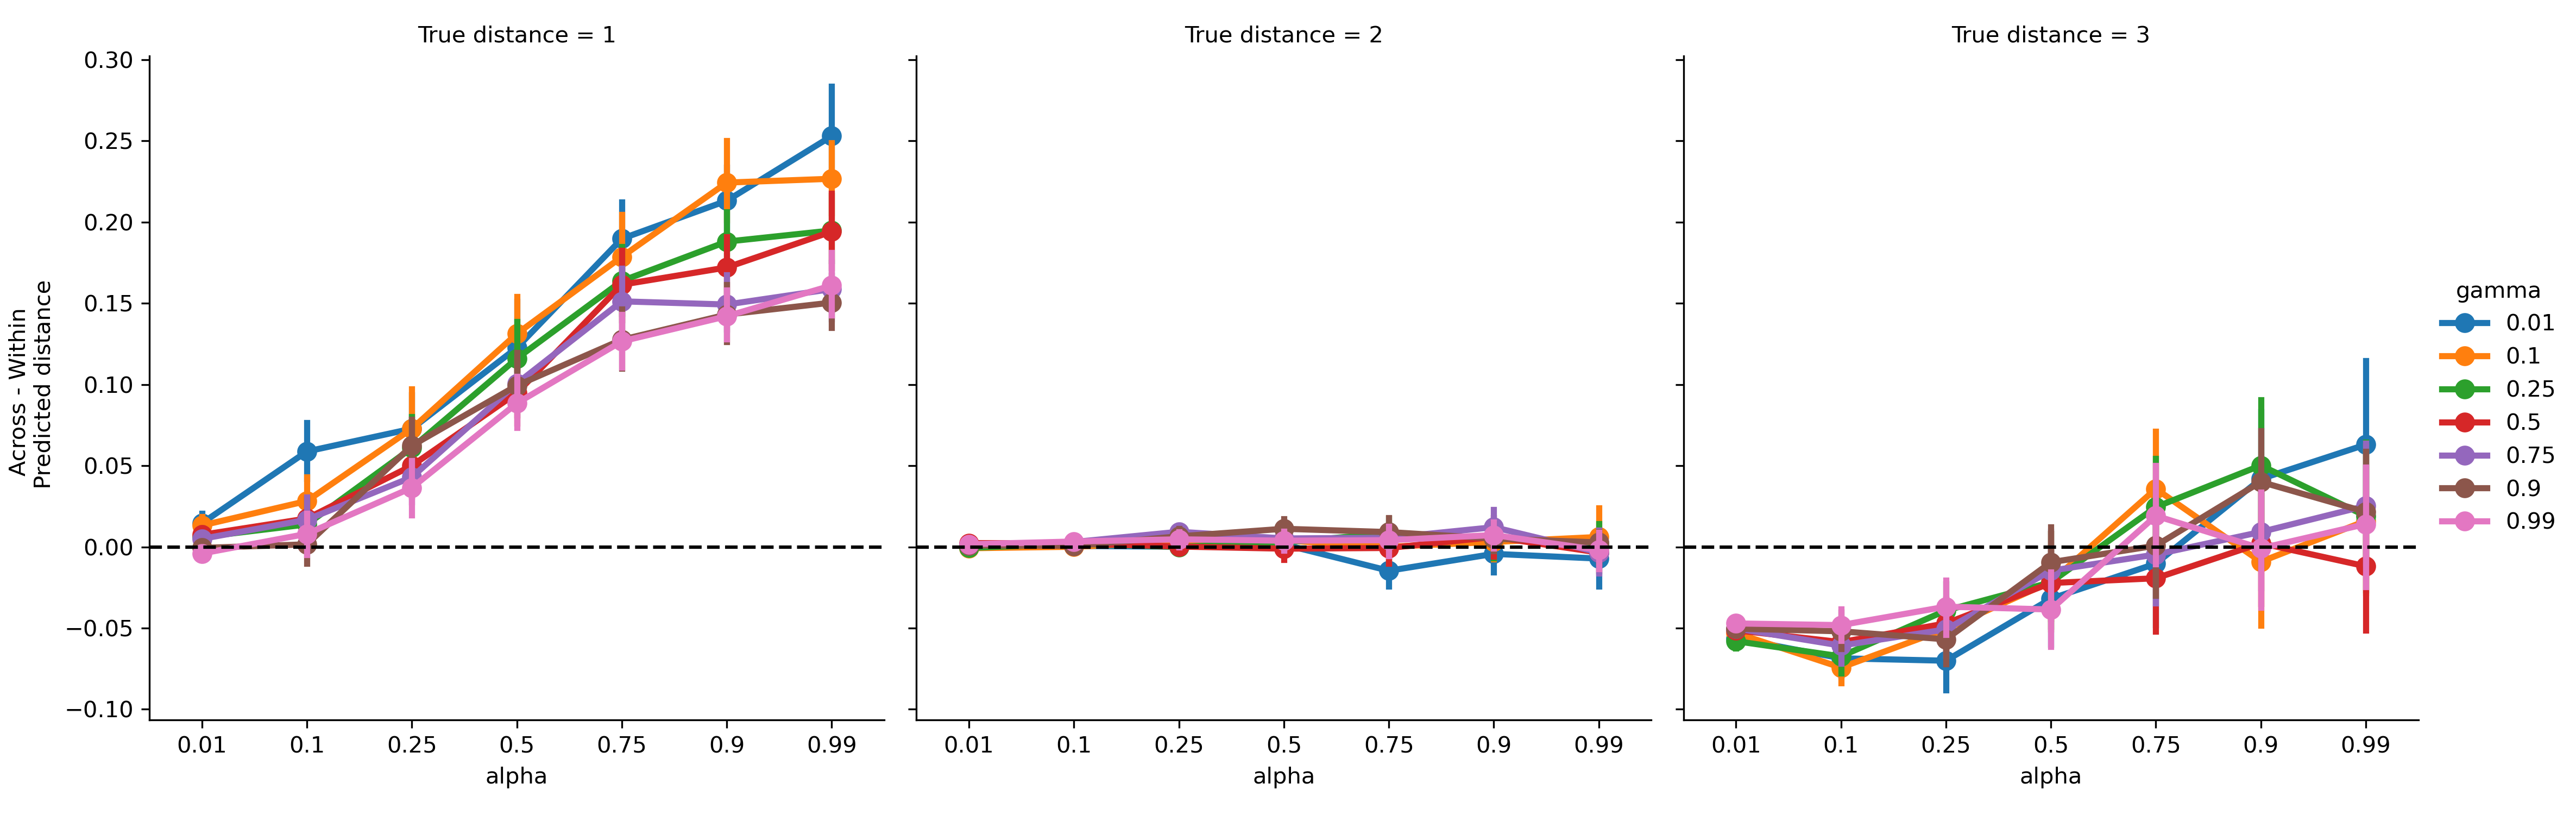
\includegraphics[width = \textwidth]{chapter_notebooks/chapter_3/figures/distance_predictions.png}
    \caption{SR predictions of distances across boundaries relative to distances within boundaries for nodes at true distance of 1, 2, and 3 and different parameter combinations.}
    \label{fig:SR-distance-estimate}
\end{figure}

SR estimate of distances is shown in Figure \ref{fig:SR-distance-estimate}. Simulations predict that while boundary nodes themselves get perceptually farther with increased discount rate, neither of the node-pairs at distance 2 or 3 that involve boundary nodes reliably show an increased cross-cluster distance. \ac{For remote nodes (which are involved in nodes at distance 3), some parameter combinations may lead to cross cluster transitions being perceived as closer.}

% \begin{figure}
%     \centering
%     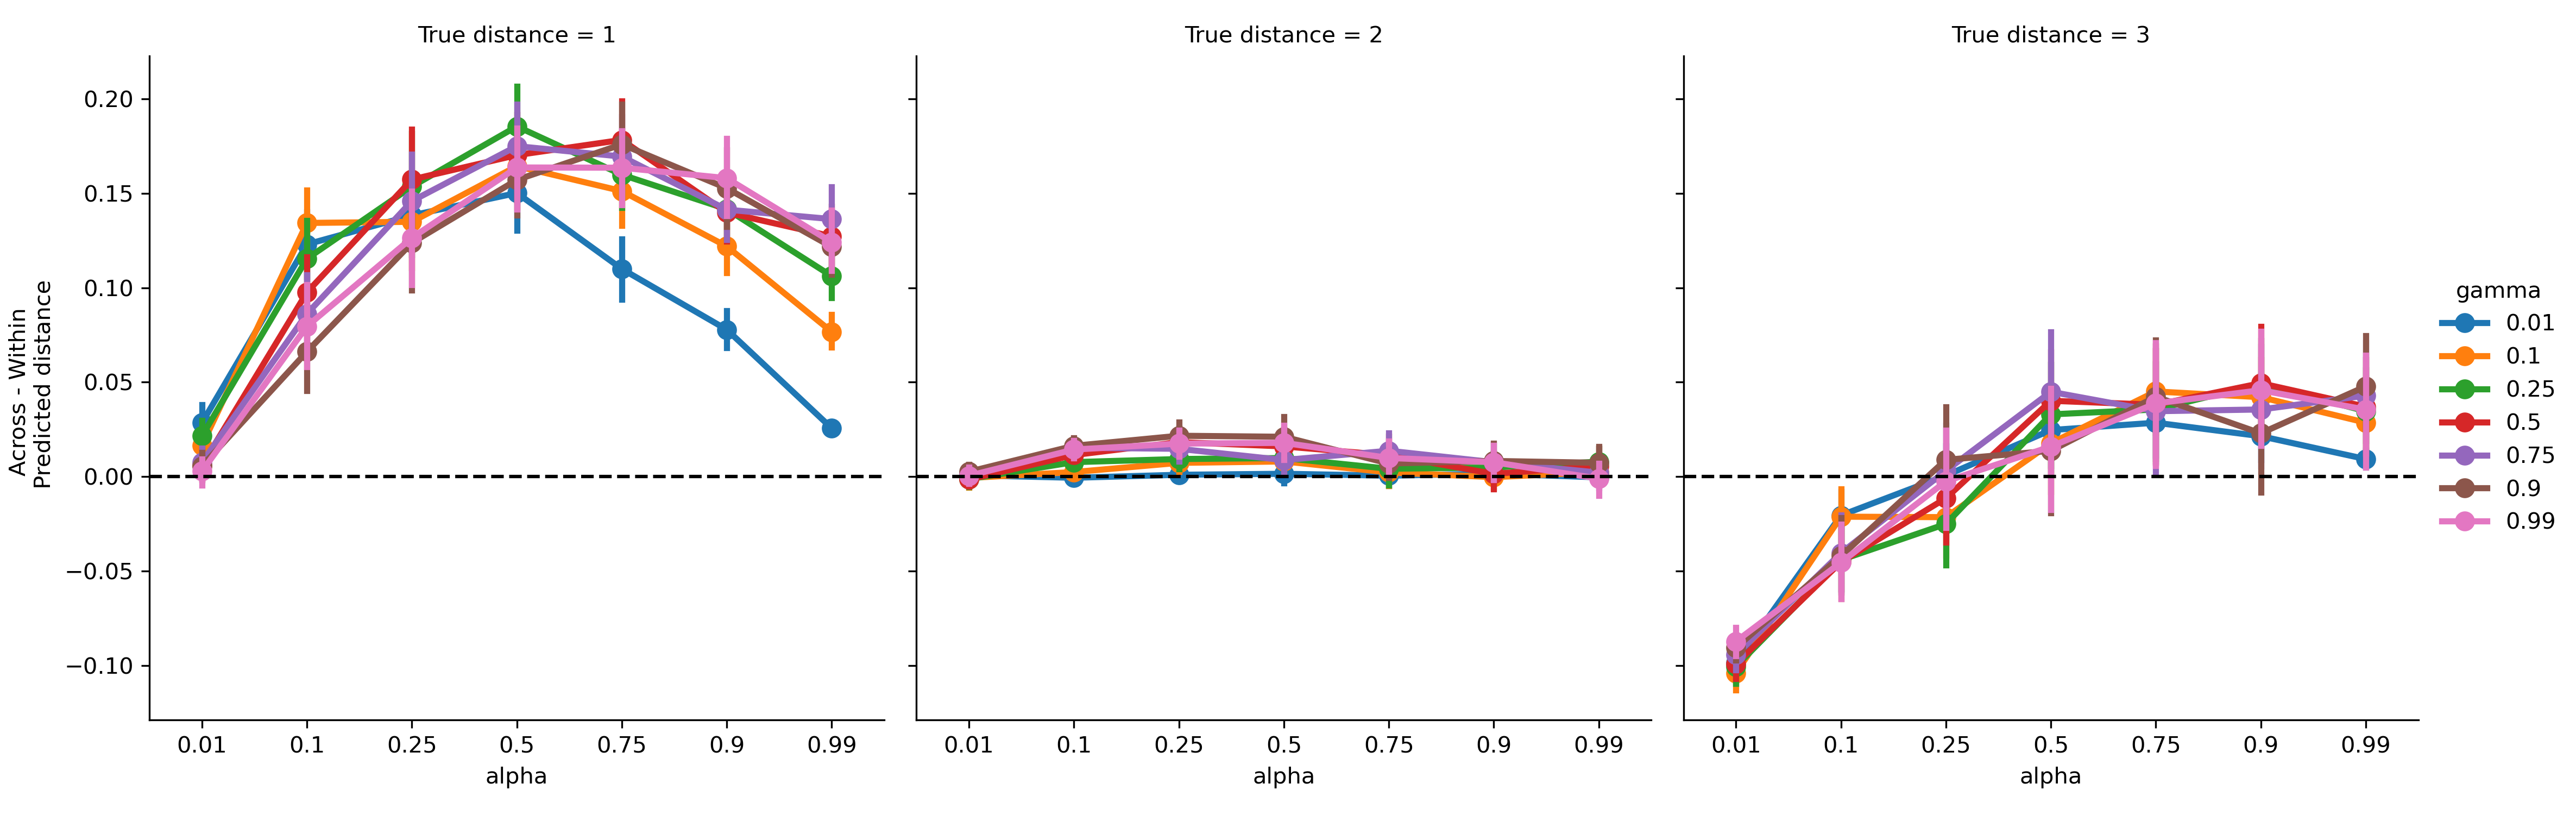
\includegraphics[width = \textwidth]{chapter_notebooks/chapter_3/figures/distance_predictions_entropyboost.png}
%     \caption{SR predictions of distances across boundaries when boosted by node entropies relative to distances within boundaries for nodes at true distance of 1, 2, and 3 and different parameter combinations.}
%     \label{fig:SR-distance-estimate-entropy-boost}
% \end{figure}

% \st{However, in a typical experience of the random walk, participants are shown to be slow at responding to boundary nodes both due to higher entropy at boundary nodes (from chapter \ref{chapter-2-walk-lengths-modulate-statistical-learning}) and previously shown increased response times during transitions across temporal clusters \parencite{lynn2020abstract,kahn2018network}. On average, a participant would typically spend more time at boundary nodes than non-boundary nodes thereby leading to increased perceived \textit{time} while crossing boundary nodes relative to staying within the cluster. Following the findings in chapter \ref{chapter-2-walk-lengths-modulate-statistical-learning}, this increased perceived time can be modeled through entropy difference between boundary and non-boundary nodes based on learned SR representations. This slowdown is simulated by multiplying average SR entropy of boundary nodes where they transitions cross boundaries and by multiplying the average SR entropy of non-boundary nodes where transitions stay within a cluster. predictions of differences in perceived distance are shown in figure \ref{fig:SR-distance-estimate-entropy-boost}.}


\ac{This SR framework predicts that neighboring} boundary nodes themselves appear farther from each other relative to nodes within a cluster from that cluster's boundary node. \ac{In fact, the SR also makes a stronger prediction that for no combination of parameters, the neighboring boundary nodes should be perceived closer to each other than a boundary node and its non-boundary neighbor. This prediction of the model is in line with past findings in explicit event boundary literature where events across boundaries are perceived to be farther from each other than event within the boundaries \parencite{heusser2018perceptual,ezzyat2011constitutes}.} 

Model predictions at other distances are mixed and dependent on parameters that allow learning of the SR. \ac{Nevertheless, the SR predicts that stimuli associated with cross cluster nodes at distance 2 should be neither perceived as closer nor farther relative to stimuli associated with within cluster nodes at distance 2. On the other hand, cross cluster nodes at distance 3 may be perceived closer or farther from each other relative to within-cluster nodes at distance 3 depending on the parameter of the SR model. These predictions are in contrast with findings in explicitly operationalized event boundary literature where stimuli presented across boundary events are perceived to be farther from each other. \parencite{heusser2018perceptual,ezzyat2011constitutes}.}

The next experiment thus tests 1) whether the typical finding of increased perceived separation between cross cluster nodes (relative to within cluster nodes) is replicated in implicitly operationalized event boundary paradigms and \ac{2) Whether SR continues to be a reasonable framework to understand the representations of implicit event boundaries.} An increased cross-cluster distance observed for nodes at distances of 2 or a decreased cross-cluster distance for nodes at true distance of 1 will serve as evidence \textit{against} the current formulation of the SR model's role in estimating temporal distances. 

\subsection{Methods}
\subsubsection*{Participants}
48 undergraduate students at the University of Massachusetts Amherst participated in this study. Participants were at least 18 years of age and were compensated via course credit. All study procedures were approved by the University Institutional Review Board. Data from 3 participants who did not complete the study were discarded from further analyses. No apriori statistical power analyses was computed to estimate sample sizes. Sample sizes were determined by rough equivalence from prior studies \parencite{heusser2018perceptual,dubrow2013influence}. 

\subsubsection*{Stimuli}
\ac{The same polygon stimuli used in the previous experiment were used for this experiment as well. For each participant, 12 random polygon stimuli wer chosen from the set of 300.}

\subsubsection*{Design and Procedures}
Participants were randomly assigned to either a structured exposure or an unstructured exposure group. The overall experimental procedures were the same across both groups. \ac{The experiment consisted of 2 phases, an `exposure' phase where participants made judgments about the orientation of the polygons and a `distance judgment' phase where participants went through a choice task making judgments about relative distance of the stimuli they saw during the exposure phase.}

Participants were first introduced to 10 randomly generated polygons and informed that these polygons are in their canonical orientation. Participants were asked to study these carefully and remember their orientations as they will make judgments about the orientation of these polygons in the coming phase. During the exposure phase, participants were shown one polygon at a time from the set of 10 they were introduced to. On each trial, the polygon was either rotated by 90 degrees or shown in its canonical orientation. Participants were asked to judge whether the polygon is rotated or not. 

The order of trials in exposure phase was determined based on a participant's group. 27 participants in the structured exposure condition were exposed to a stimulus stream generated by a random walk through the graph in figure \ref{fig:two_module_graph}. 18 participants in the unstructured exposure condition were shown a stimulus stream generated by randomly choosing any of the 10 polygons to be shown on any trial. The exposure phase lasted for 300 trials or 30 minutes, whichever came first. Participants were provided with an opportunity to take a self-paced break after 150 trials. 

\begin{figure}
    \centering
    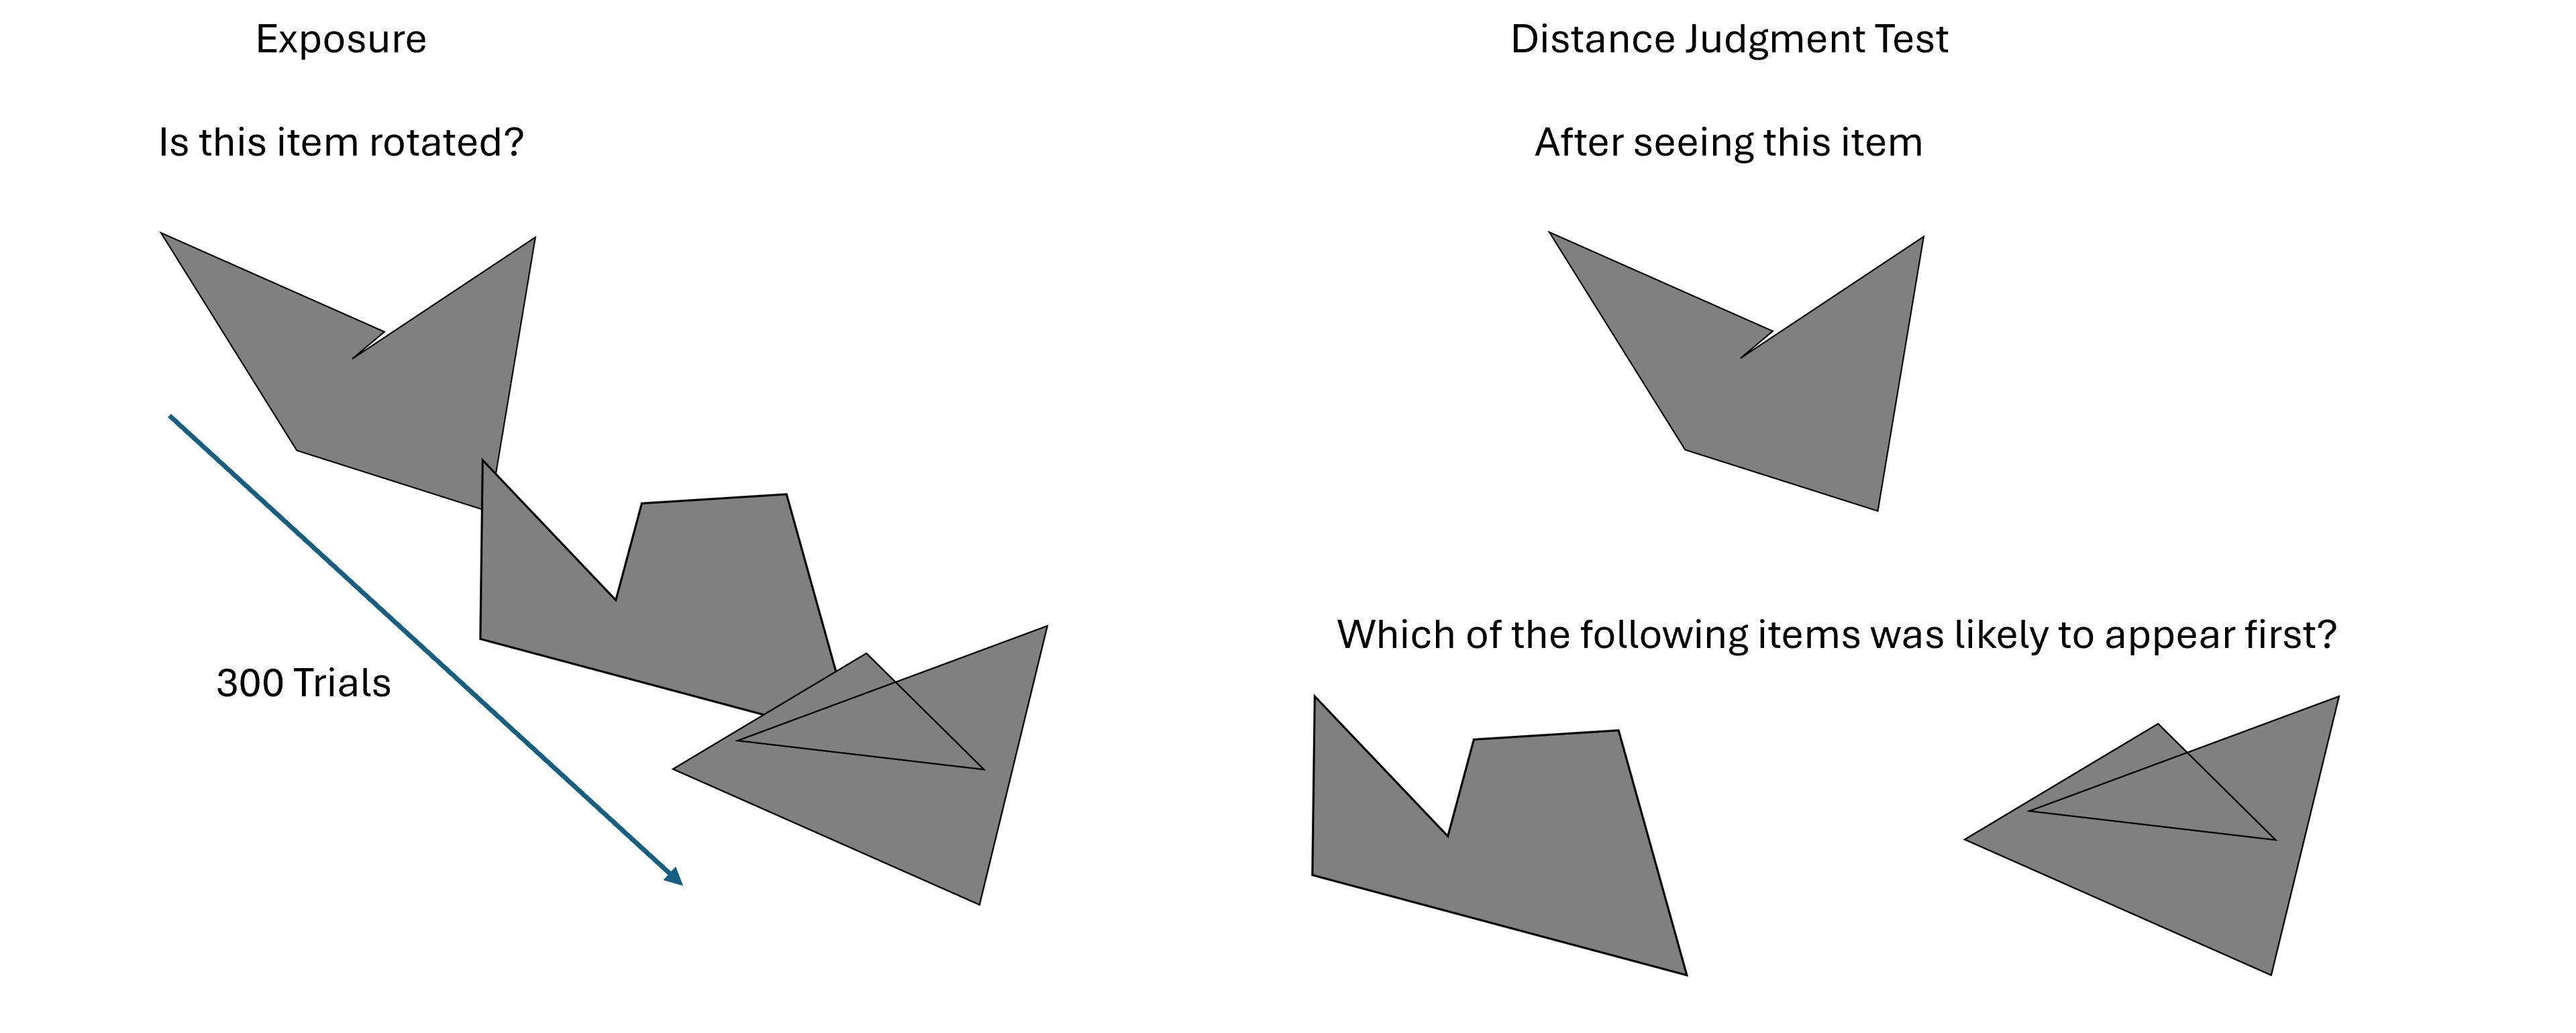
\includegraphics[width = \textwidth]{chapter_notebooks/chapter_3/figures/exp3_design.png}
    \caption{Design schematic for experiment 2b. After exposure through the graph structured (based on a random walk through the connected nodes or a random selection between all 15 nodes), participants went through a distance judgment phase}
    \label{fig:exp3-design}
\end{figure}


During the test phase, participants were shown a triplet of polygons (see Figure \ref{fig:exp3-design}). For each top polygon, participants were asked which of the bottom polygons was likely to appear first after seeing the polygon at the top in the stream they had experienced during exposure. The distance judgment phase lasted for 20 trials where 10 trials consisted of the critical pairs (examples listed in the previous section) and 10 filler trials were based on randomly generated (non repeated) triplets. Responses to these filler trials were not analyzed.

\subsection{Results}

\begin{figure}
    \centering
    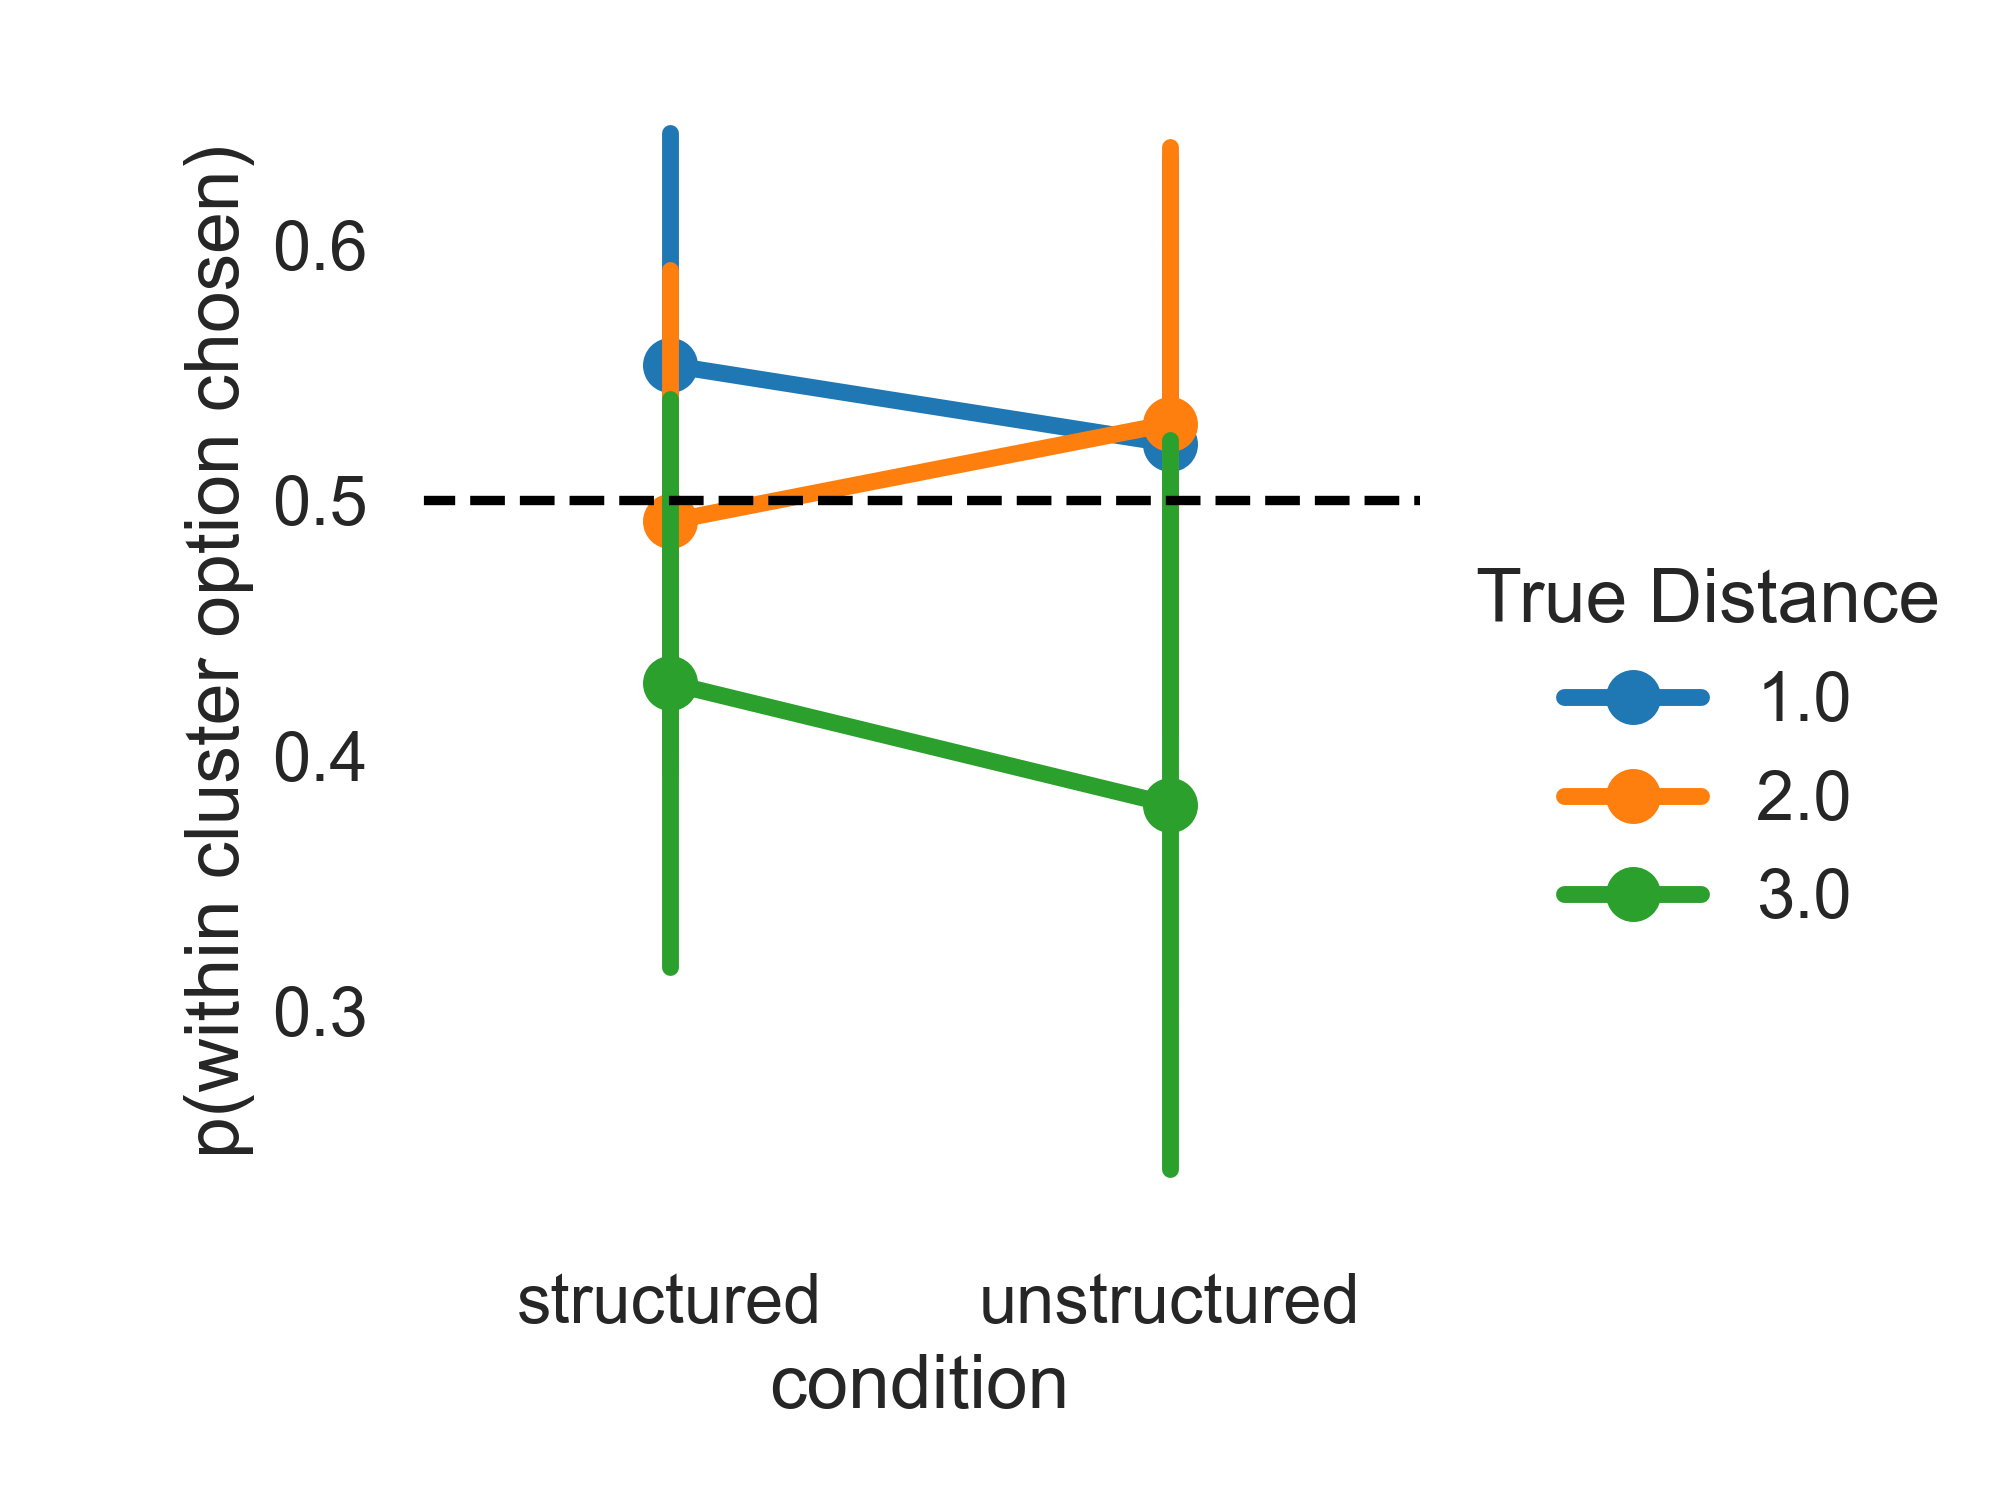
\includegraphics[width = \textwidth]{chapter_notebooks/chapter_3/figures/exp3_choice_results.png}
    \caption{Proportion of trials where the within cluster option was chosen when the distance between and within clusters were equal (ranging from a distance of 1, 2, and 3 connections).}
    \label{fig:exp3-choice-results}
\end{figure}


Figure \ref{fig:exp3-choice-results} provides an overview of the proportion of choices participants made to indicate a within cluster item is closer to the top item than a between cluster item. Descriptive statistics in Table \ref{tab:exp3-choice-stats}. \ac{For all conditions, response probabilities were largely at chance indicating that within-cluster option did not appear closer to most participants relative to the across-cluster option regardless of the true distance. To assess this statistically, a hierarchical Bayesian Model was fit the within cluster choice probability as follows:} 
\begin{equation}
    \begin{aligned}
        p(within\ option\ chosen) ~ 0 + true\ distance:condition + (1|participant)
    \end{aligned}
\end{equation}

Figure \ref{fig:exp3-bayesmodel_results} provides a bayesian estimate of the difference in proportion of within cluster option chosen relative to the between cluster option when participants are exposed to a structured, random walk presentation order compared to when they were exposed to unstructured presentation order. \mh{For all distances, there is no apparent difference between these proportions in either direction. The within cluster option was chosen more often in the structured exposure relative to unstructured exposure with 65.53\% probability for true distance of 1, 31.92\% probability for true distance of true and 66.38\% probability for a true distance of 3. Since 95\% HDIs for all True distances include 0, the structured exposure did not lead to higher selection of within cluster stimuli as being closer.}


\begin{figure}
    \centering
    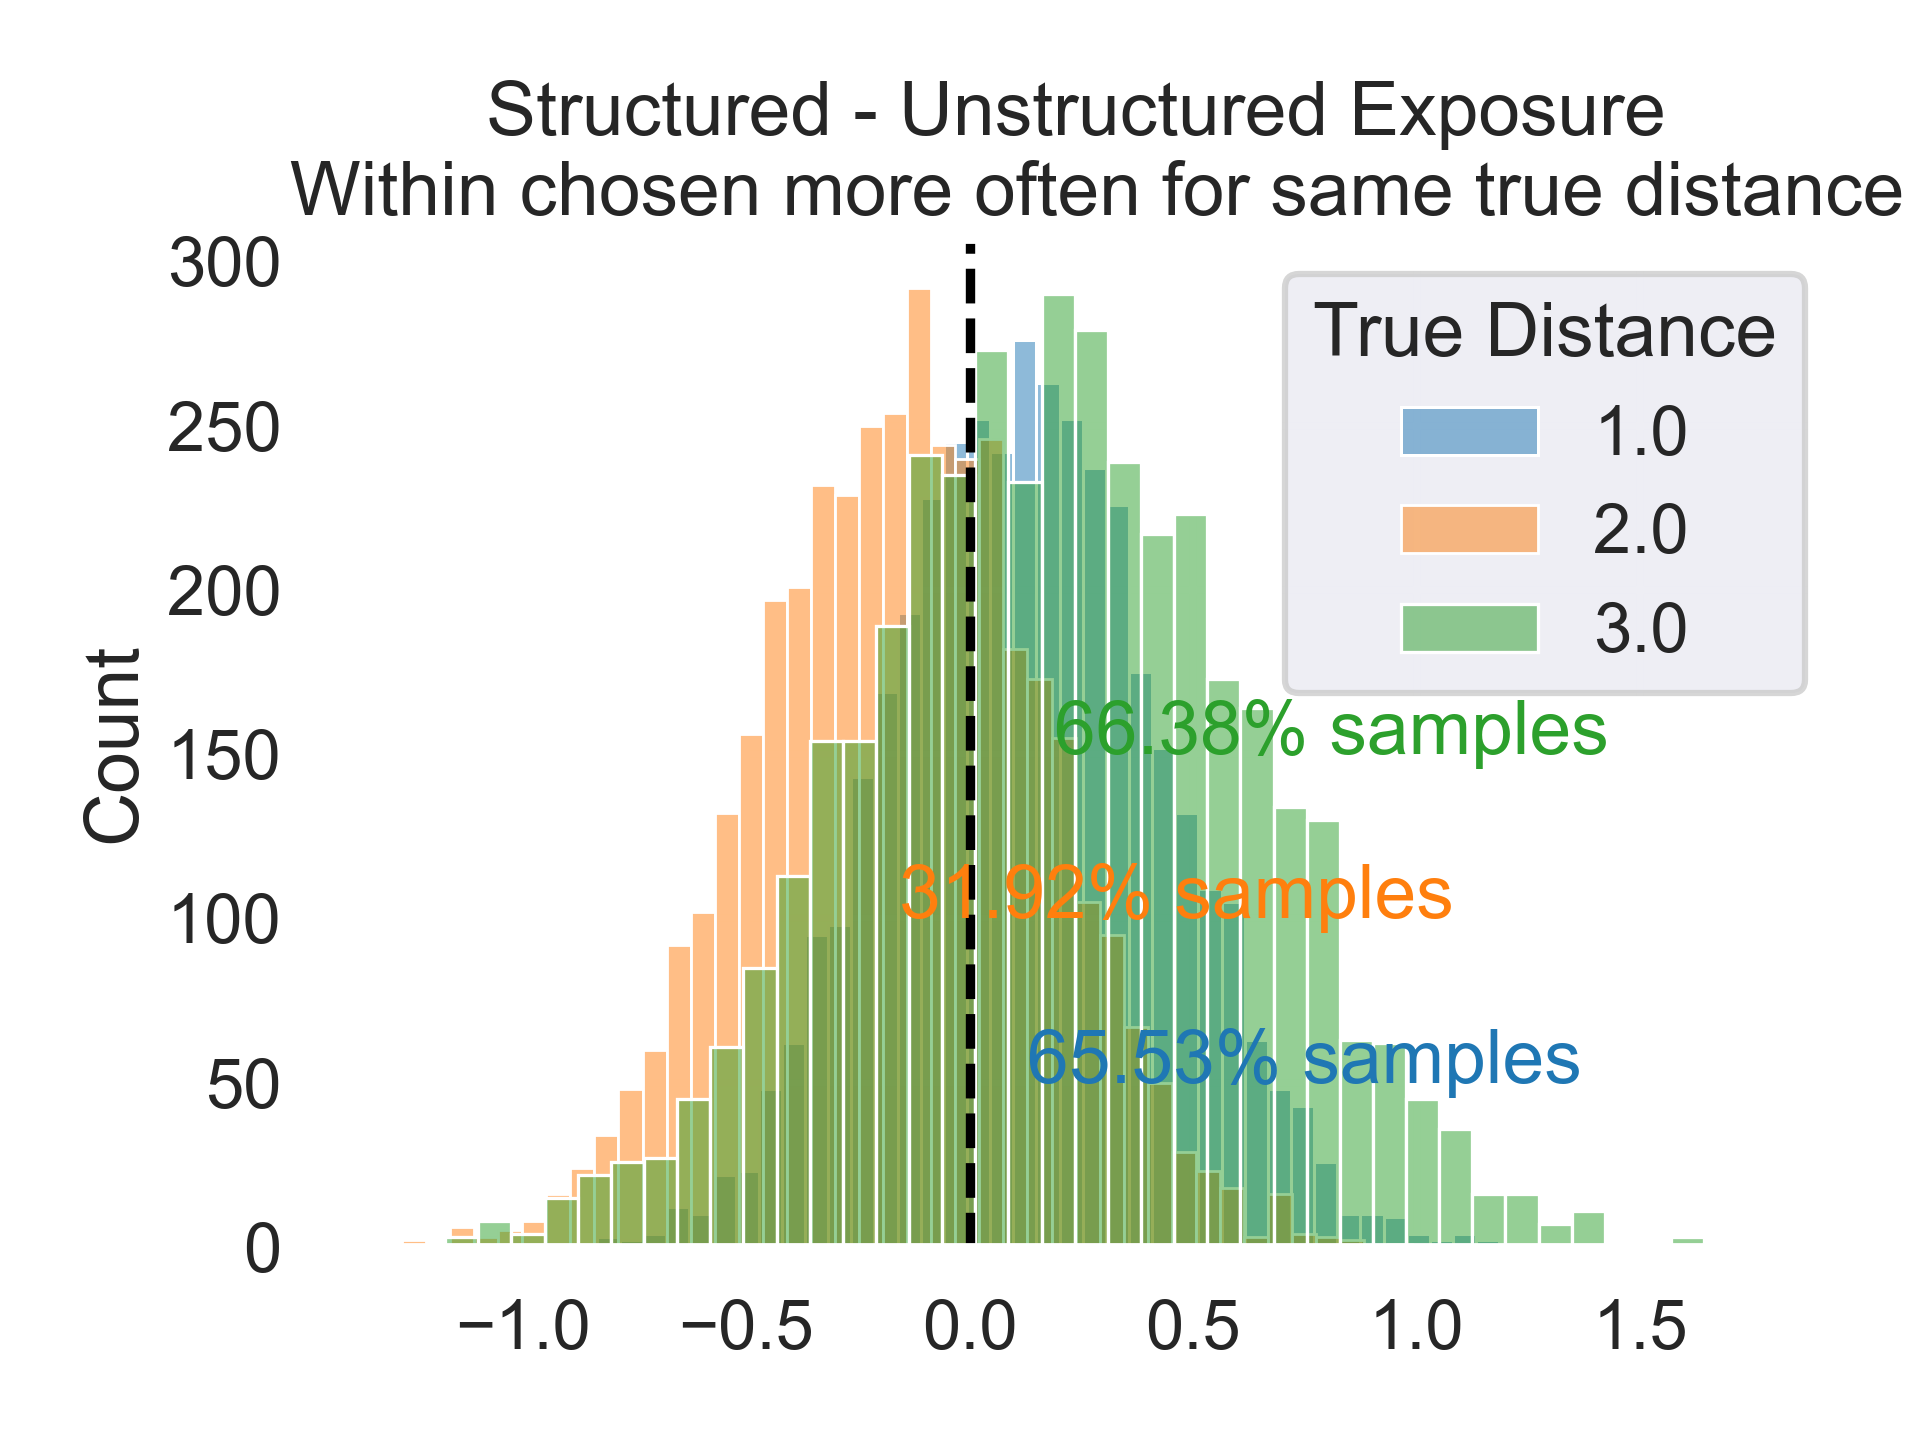
\includegraphics[width = \textwidth]{chapter_notebooks/chapter_3/figures/exp3_bayesmodel_results.png}
    \caption{Posterior estimates of the differences between structured and unstructured exposure condition for the proportion of times when the option within cluster was chosen more often as being closer than the option across the cluster at the same shortest distance.}
    \label{fig:exp3-bayesmodel_results}
\end{figure}

\begin{table}
    \centering
    \begin{tabular}{llrr}
        \toprule
         &  & \multicolumn{2}{r}{within chosen} \\
         &  & mean & std \\
        condition & true distance &  &  \\
        \midrule
        \multirow[t]{3}{*}{structured} & 1.0 & 0.565 & 0.497 \\
         & 2.0 & 0.505 & 0.501 \\
         & 3.0 & 0.450 & 0.500 \\
        \cline{1-4}
        \multirow[t]{3}{*}{unstructured} & 1.0 & 0.528 & 0.501 \\
         & 2.0 & 0.533 & 0.501 \\
         & 3.0 & 0.521 & 0.503 \\
        \cline{1-4}
        \bottomrule
    \end{tabular}
     \caption{Proportions of trials where within cluster option at the same distance as the between cluster option was chosen.}   
     \label{tab:exp3-choice-stats}
\end{table}


\section{Discussion}

The primary goal of this chapter was to test whether findings in classical explicitly operationalized event boundary literature replicate when boundaries are operationalized implicitly, through temporal statistics. Shared properties between these two boundaries imply shared representations in memory thereby providing a framework for future research to study shared algorithmic processes that lead to formation of event boundaries. 

\mh{In Experiment 2a, I test whether similar to findings in the explicitly operationalized event boundary literature (where boundary events are perceptually different from the ongoing stream of events), participants remember implicitly operationalized boundar events (where boundary events are not perceptually different but serve as a gateway to a different cluster defined by temporal co-occurences). I propose an SR based framework to model potential differences in memory between implicit boundary and non-boundary events. The SR based framework predicts that since boundary nodes carry higher information about the structure of the environment they will be remembered better than the non-boundary nodes. Findings of Experiment 2a support this prediction. Specifically, implicit boundary nodes have a higher drift rate than non-boundary nodes.}

DDM is one (highly successful) model of memory that incorporates response time distributions along with choices. Several other sequential sampling models can be used in this formulation to provide evidence of better memory strength for boundary items. Most notably, a direct extension of the GCM model for recognition memory is the Exemplar Based Random Walk (EBRW) model \parencite{nosofsky2011short} which assumes that evidence towards old/new recognition choice options is accumulated made in proportion to background activation of all items in memory may be extended to incorporate node entropies in its evidence accumulation process. For example, higher entropy (typical for stimuli at boundary nodes in structured random walks relative to non-boundary nodes) may lead to increased activation of boundary stimuli relative to background activation thereby leading to better recognition. Further work is needed to understand how extensions to other choice reaction time models can be extended to incorporate effects of temporal order.

\mh{The effect of structured exposure on identifying new stimuli is intriguing (Figure \ref{fig:ddm-drift-rates}). Higher drift rates for new items in the structured condition relative to the unstructured condition may imply support for event integration at boundary nodes \parencite{zacks2007event}. Structure may allow extraction of higher order knowledge (segmented at boundary stimuli) and hence makes it easier to identify events that do not belong to that structure. Such SR framework may help future investigation should aim to diagnose the underlying cognitive processes that lead to recognition of new stimuli.}

\ac{\textbf{Finally, model simulations in Experiment 2a have followed from simplifying assumptions about mental processes at test. In particular, the assumption of a stable context for all test items warrants a mention. In most context-based recognition memory models, and especially global matching models, items at test are often said to reinstate the context in which they were studied \parencite{polyn2009context,murdock1997context, osth2020global, hicks2006remembering, cox2020similarity}. This assumption is relaxed for recognition memory simulations for Experiment 2b, thereby implicitly assuming that context reinstatement does not play a role in the boundary memory effect. While the comparison between unstructured and structured exposure across participants and between boundary and non-boundary stimuli within participants provides support for an internal validity of this assumption, future research should aim to account for context reinstatements at test items for similar implicit event boundary models. Indeed, event cognition literature suggests explicit event boundaries serve as points of replay \parencite{hahamy2023human} and points at which memory is scanned \parencite{michelmann2023evidence}. It is likely that recall of boundary events reinstates surrounding context and future work should thus investigate the role of SR-based context reinstatement on recall performance.}}. 

\ac{\textbf{Similarly, the model simulations also assume that the effect of boundary entropy is on the memory strength parameter. As stated above, it is possible that boundaries are not necessarily remembered better but reinstatement of context, which the boundaries represent better, is what leads to improved recall. Future work should also investigate the validity of the assumption of memory strength being impacted by boundary node. Regardless of why boundary nodes are remembered better, the fact that they are as shown in the current work, is an important step in deriving common representations between implicit and explicit event boundaries.}}

\mh{In the Experiment 2b, I aim to test 1) Whether similar to explicitly operationalized boundaries, implicit boundaries also temporally stretch events in memory, and 2) Whether the SR framework continues to be a reliable model of representation of implicit boundaries. The SR model allows us to simultaneously test both these hypothesis for a graph structure with two modules and remote nodes (Figure \ref{fig:two_module_graph}). Specifically, for across-boundary nodes at distance 2 or 3, the model predicts no reliable increase in selection of within boundary nodes as being closer. On the other hand, within boundary nodes should be selected more often as being closer than across boundary nodes for nodes at distance of 1. Furthermore, the model predicts that for nodes at distances 1 or 2, across boundary nodes should \textit{not} be chosen as being closer; thereby providing an avenue for the SR model to be falsified. The model further predicts that for some parameter values, cross cluster nodes may be chosen as closer than within cluster remote nodes, a prediction that suggests that implicitly operationalized event boundaries may not follow similar behavioral properties as explicitly operationalized boundaries. }

\mh{Findings in Experiment 3b suggest that implicitly operationalized event boundaries may not share properties with explicitly operationalized event boundaries -- participants do not reliably select the within cluster stimuli to be closer relative to across cluster stimuli at the same distance. Furthermore, the lack of this within-across cluster effect for nodes at distance 1 indicates lack of support for the SR model framework that's used for predictions. Nevertheless, since for distances 1 and 2, across cluster stimuli were \textit{not} chosen more often than within cluster stimuli, the SR model was not falsified.}

\mh{The lack of support for model predictions in experimental findings provides an additional avenue for further testing of this SR framework. While SR allows for small effects at distance 1 for lower learning rates and discount parameters, the lack of the observed effect may simply reflect a harder-to-detect small effect. The model can be further falsified through experimental designs that allow for varying idiosynchratic learning and discount rate parameters. For example, providing participants information about an existing temporal structure may lead to an increased learning rate or discount parameters. Lack of increased selection of within cluster option as being closer in such a case would provide a stronger evidence against the SR framework. Finally, future work should also incorporate other context models such as the TCM \parencite{howard2005temporal,polyn2009context} to directly compare them with the current SR framework \parencite{gershman2012successor} their predictions on such distance judgment tasks.}

\mh{Finally, both experiments used specific graph structures to investigate possible shared properties of implicit and explicit event boundaries. While the SR model makes a theoretical prediction of similar findings across topological variations, future work should also attempt to identify if altering the properties of various graph topologies can lead to different experimental observations.}

\section{Conclusion}
In this chapter, I aimed to assess whether implicitly operationalized boundaries lead to the same behavioral properties as explicitly operationalized boundaries. Implicitly operationalized boundaries are indeed remembered better. However, evidence from the distance judgment is mixed. Future experimental paradigms should investigate whether more regular graphs (without remote nodes, for example) lead to the increased cross boundary distance. 
